%  LaTeX support: latex@mdpi.com 
%  For support, please attach all files needed for compiling as well as the log file, and specify your operating system, LaTeX version, and LaTeX editor.

%=================================================================
\documentclass[entropy,article,submit,pdftex,moreauthors]{Definitions/mdpi} 
% For posting an early version of this manuscript as a preprint, you may use "preprints" as the journal and change "submit" to "accept". The document class line would be, e.g., \documentclass[preprints,article,accept,moreauthors,pdftex]{mdpi}. This is especially recommended for submission to arXiv, where line numbers should be removed before posting. For preprints.org, the editorial staff will make this change immediately prior to posting.

%=================================================================
% MDPI internal commands
\firstpage{1} 
\makeatletter 
\setcounter{page}{\@firstpage} 
\makeatother
\pubvolume{1}
\issuenum{1}
\articlenumber{0}
\pubyear{2022}
\copyrightyear{2022}
%\externaleditor{Academic Editor: Firstname Lastname}
\datereceived{} 
%\daterevised{} % Only for the journal Acoustics
\dateaccepted{} 
\datepublished{} 
%\datecorrected{} % Corrected papers include a "Corrected: XXX" date in the original paper.
%\dateretracted{} % Corrected papers include a "Retracted: XXX" date in the original paper.
\hreflink{https://doi.org/} % If needed use \linebreak
%\doinum{}
%------------------------------------------------------------------
% The following line should be uncommented if the LaTeX file is uploaded to arXiv.org
%\pdfoutput=1

%=================================================================
% Add packages and commands here. The following packages are loaded in our class file: fontenc, inputenc, calc, indentfirst, fancyhdr, graphicx, epstopdf, lastpage, ifthen, lineno, float, amsmath, setspace, enumitem, mathpazo, booktabs, titlesec, etoolbox, tabto, xcolor, soul, multirow, microtype, tikz, totcount, changepage, attrib, upgreek, cleveref, amsthm, hyphenat, natbib, hyperref, footmisc, url, geometry, newfloat, caption

% \usepackage{mathptmx}      % use Times fonts if available on your TeX system
%
% insert here the call for the packages your document requires
%\usepackage{latexsym}
\newcommand\hmmax{0}
\newcommand\bmmax{0}


\usepackage{dcolumn}% Align table columns on decimal point
\usepackage{bm}% bold math
\setlength{\marginparwidth}{2cm}
\usepackage{changes}
\usepackage{bbm}
%\usepackage[mathlines]{lineno}% Enable numbering of text and display math
%\linenumbers\relax % Commence numbering lines
\usepackage{mathptmx}
\usepackage{amssymb}
\usepackage{statmath}
\usepackage{enumitem}
\usepackage{mathtools}
\usepackage{siunitx}
\DeclarePairedDelimiter\ceil{\lceil}{\rceil}
%
% please place your own definitions here and don't use \def but
\newcommand{\mytilde}{\raise.17ex\hbox{$\scriptstyle\mathtt{\sim}$}}

%=================================================================
%% Please use the following mathematics environments: Theorem, Lemma, Corollary, Proposition, Characterization, Property, Problem, Example, ExamplesandDefinitions, Hypothesis, Remark, Definition, Notation, Assumption
%% For proofs, please use the proof environment (the amsthm package is loaded by the MDPI class).

%=================================================================
% Full title of the paper (Capitalized)
\Title{Spike spectra for recurrences}

% MDPI internal command: Title for citation in the left column
\TitleCitation{Spike spectra for recurrences}

% Author Orchid ID: enter ID or remove command
\newcommand{\orcidauthorA}{0000-0002-9943-5391} % Add \orcidA{} behind the author's name
\newcommand{\orcidauthorB}{0000-0001-6643-9508} % Add \orcidB{} behind the author's name
\newcommand{\orcidauthorC}{0000-0003-1437-7039} % Add \orcidB{} behind the author's name

% Authors, for the paper (add full first names)
\Author{K. Hauke Kraemer $^{1,}$*\orcidA{}, Frank Hellmann $^{1,}$, Mehrnaz Anvari $^{1}$\orcidB{}, J\"urgen Kurths $^{1,2,4}$ and Norbert Marwan $^{1,2,3,}$*\orcidC{}}

%\longauthorlist{yes}

% MDPI internal command: Authors, for metadata in PDF
\AuthorNames{K. Hauke Kraemer, Frank Hellmann, Mehrnaz Anvari, J\"urgen Kurths and Norbert Marwan}

% MDPI internal command: Authors, for citation in the left column
\AuthorCitation{Kraemer, K.H..; Hellmann, F.; Anvari M.; Kurths, J.; Marwan, N.}
% If this is a Chicago style journal: Lastname, Firstname, Firstname Lastname, and Firstname Lastname.

% Affiliations / Addresses (Add [1] after \address if there is only one affiliation.)
\address{%
$^{1}$ \quad Potsdam Institute for Climate Impact Research, Member of the Leibniz Association, 14473 Potsdam, Germany\\
$^{2}$ \quad Institute of Physics and Astronomy, University of Potsdam, 14476 Potsdam, Germany\\
$^{3}$ \quad Institute of Geosciences, University of Potsdam, 14476 Potsdam, Germany\\
$^{4}$ \quad Institute of Physics, Humboldt Universit\"at zu Berlin, 12489 Berlin, Germany}

% Contact information of the corresponding author
\corres{Correspondence: hauke\_kraemer@hotmail.com; marwan@pik-potsdam.de}

% Current address and/or shared authorship
%\firstnote{Current address: Affiliation 3.} 
%\secondnote{These authors contributed equally to this work.}
% The commands \thirdnote{} till \eighthnote{} are available for further notes

%\simplesumm{} % Simple summary


% Abstract (Do not insert blank lines, i.e. \\) 

\abstract{In recurrence analysis, the $\tau$-recurrence rate encodes the periods of the cycles of the underlying high-dimensional time series. 
It, thus, plays a similar role to the autocorrelation for scalar time-series in encoding temporal correlations. 
However, its Fourier decomposition does not have a clean interpretation. 
Thus, there is no satisfactory analogue to the power spectrum in recurrence analysis. 
We introduce a novel way to decompose the $\tau$-recurrence rate using an over-complete basis of Dirac combs together with a sparsity regularization. 
We show that this decomposition, the \textit{inter-spike spectrum}, naturally provides an analogue to the power spectrum for recurrence analysis in the sense that it reveals the dominant periodicities of the underlying time series. 
We show that the inter-spike spectrum correctly identifies patterns and transitions in the underlying system in a wide variety of examples and is robust to measurement noise.}


% Keywords
\keyword{Decomposition; Frequency Analysis; Recurrence Analysis; Bifurcations}
\PACS{05.45.Tp, 05.90.+m, 89.90.+n, 02.70.Uu, 05.10.Ln, 05.45.-a, 05.45.Ac}


%%%%%%%%%%%%%%%%%%%%%%%%%%%%%%%%%%%%%%%%%%
\begin{document}

\section{Introduction}\label{sec_tau_rr_intro}

The dynamics of complex systems as provided by measured time series usually show complicated and chaotic patterns.
Quantifying their recurrence features is a powerful way to describe them and to infer information about 
the type of dynamics, stability, regime changes, or couplings and synchronisation \cite{marwan2007,marwan2008epjst,webber2015}.
Even more challenging are signals which do have a heavy tailed-distribution or appear as a spike-train,
e.g., neuron firings \cite{Dummer2014,Orcioni2020}, heart beat variability \cite{marwan2002herz}, 
or extreme flood events \cite{banerjee2021}.
Deriving useful information from spike-train signals or inter-spike time series is an important
topic in data analysis in many scientific fields \cite{Kajikawa2005,Dummer2014,Orcioni2020,Canale2021}.

Recurrence plots (RPs) provide a vivid representation of complex dynamics $\vec{x}_i$ stemming from potentially high dimensional systems \cite{marwan2007}
\begin{equation}\label{eq_rp_definition}
R_{i,j}(\varepsilon) = \Theta\left(\varepsilon - D_{i,j}\right) 
= \Theta\left(\varepsilon - \| \vec{x}_i - \vec{x}_j\|\right), \qquad \vec{x} \in \mathbb{R}^d, \quad i,j \in [1,\ldots, N],
\end{equation}
with $\mathbf{R}$ the recurrence matrix, $\vec{x}_i$ the state vector at time 
$t = \Delta t \cdot i$ ($\Delta t$ the sampling time), $N$ the number of
sampling points (or length of data series), and $d$ the dimension of the system.
The crucial free parameter $\varepsilon$ is the recurrence threshold, determining what is a recurrences
and, thus, the visible structures in the RP. It can be chosen such that the recurrence rate 
$RR(\varepsilon)=N^{-2}\sum_{i,j}^N R_{i,j}(\varepsilon)$ exhibits a certain value \cite{kraemer2018}.
The simple idea to track recurring states of the $d$-dimensional trajectory $\vec{x}_i$ of the system under study not only allows for a beneficial visualization of the dynamics, 
but also for its 
quantification, using certain structures in the RP, such as diagonal or vertical lines \cite{marwan2007}. 

Some of these recurrence quantification measures, the entropy of diagonal lines and the entropy of 
recurrence times, can be related to basic characteristics of complex systems, such as the Kolmogorov-Sinai entropy \cite{march2005,baptista2010}. However, these quantifiers have a free parameter, the minimal considered line length, and 
are usually biased, due to the finite size of the RP and thickened diagonal lines, which needs to be corrected \cite{Kraemer2019}. Moreover, the mentioned statistics cannot account for 
changing regular (non-chaotic) dynamics, such as period-doubling bifurcations.

A rather simple idea is to look at the $\tau$-recurrence rate of the RP ($\tau$-RR, Eq.~\ref{eq_tau_rr}) \cite{marwan2002pla,Zbilut2008}.
This is the density of recurrence points along the diagonals of the recurrence matrix, as a function of the distance $\tau$ (sampling units) to the main diagonal:
\begin{equation}\label{eq_tau_rr}
\tau\text{-RR}(\varepsilon) = RR(\tau, \varepsilon) = \frac{1}{N-\tau} \sum_{i=1}^{N-\tau	} R_{i,i+\tau}.
\end{equation}
$\tau$-RR serves as an estimator for the probability that the system recurs after time $\tau \Delta t$, with $\Delta t$ being the sampling time of the trajectory 
$\vec{x}_i = \vec{x}(\Delta t \cdot i),\, i=1,\ldots,N$. 
It represents the period length of cycles in the data (Fig.~\ref{fig_tau_rr_spectrum_example}D).

\citet{Zbilut2008} pointed out that $\tau$-RR could be interpreted as analogous to the auto-correlation function $C(\tau)$ and, hence, via the Wiener-Khinchin theorem, provide an analogue,
``generalized'', spectral density. This is reasonable, since the average distances for a given lag $\tau$ 
\begin{equation}
\overline{D}(\tau) = \frac{1}{N-\tau}\sum_{i=1}^{N-\tau} D_{i, i+\tau}
\end{equation}
can be directly read from the distance matrix $\mathbf{D}$ and is also preserved in its thresholded version $\tau$-RR. There are clear advantages for a recurrence-derived spectral density, 
i.e., Fourier transforming (FT) $\tau$-RR (Fig.~\ref{fig_tau_rr_spectrum_example}D,E), instead 
of $C(\tau)$: There are no assumptions for stationarity or sampling, when constructing a RP.
Furthermore, since an RP can represent high-dimensional dynamics and its $\tau$-RR serves as a plug-in for $C(\tau)$, the correlation structures of higher dimensional spaces can be read from 
the recurrence-derived Fourier-spectrum.\\

\begin{figure}
 \centering
 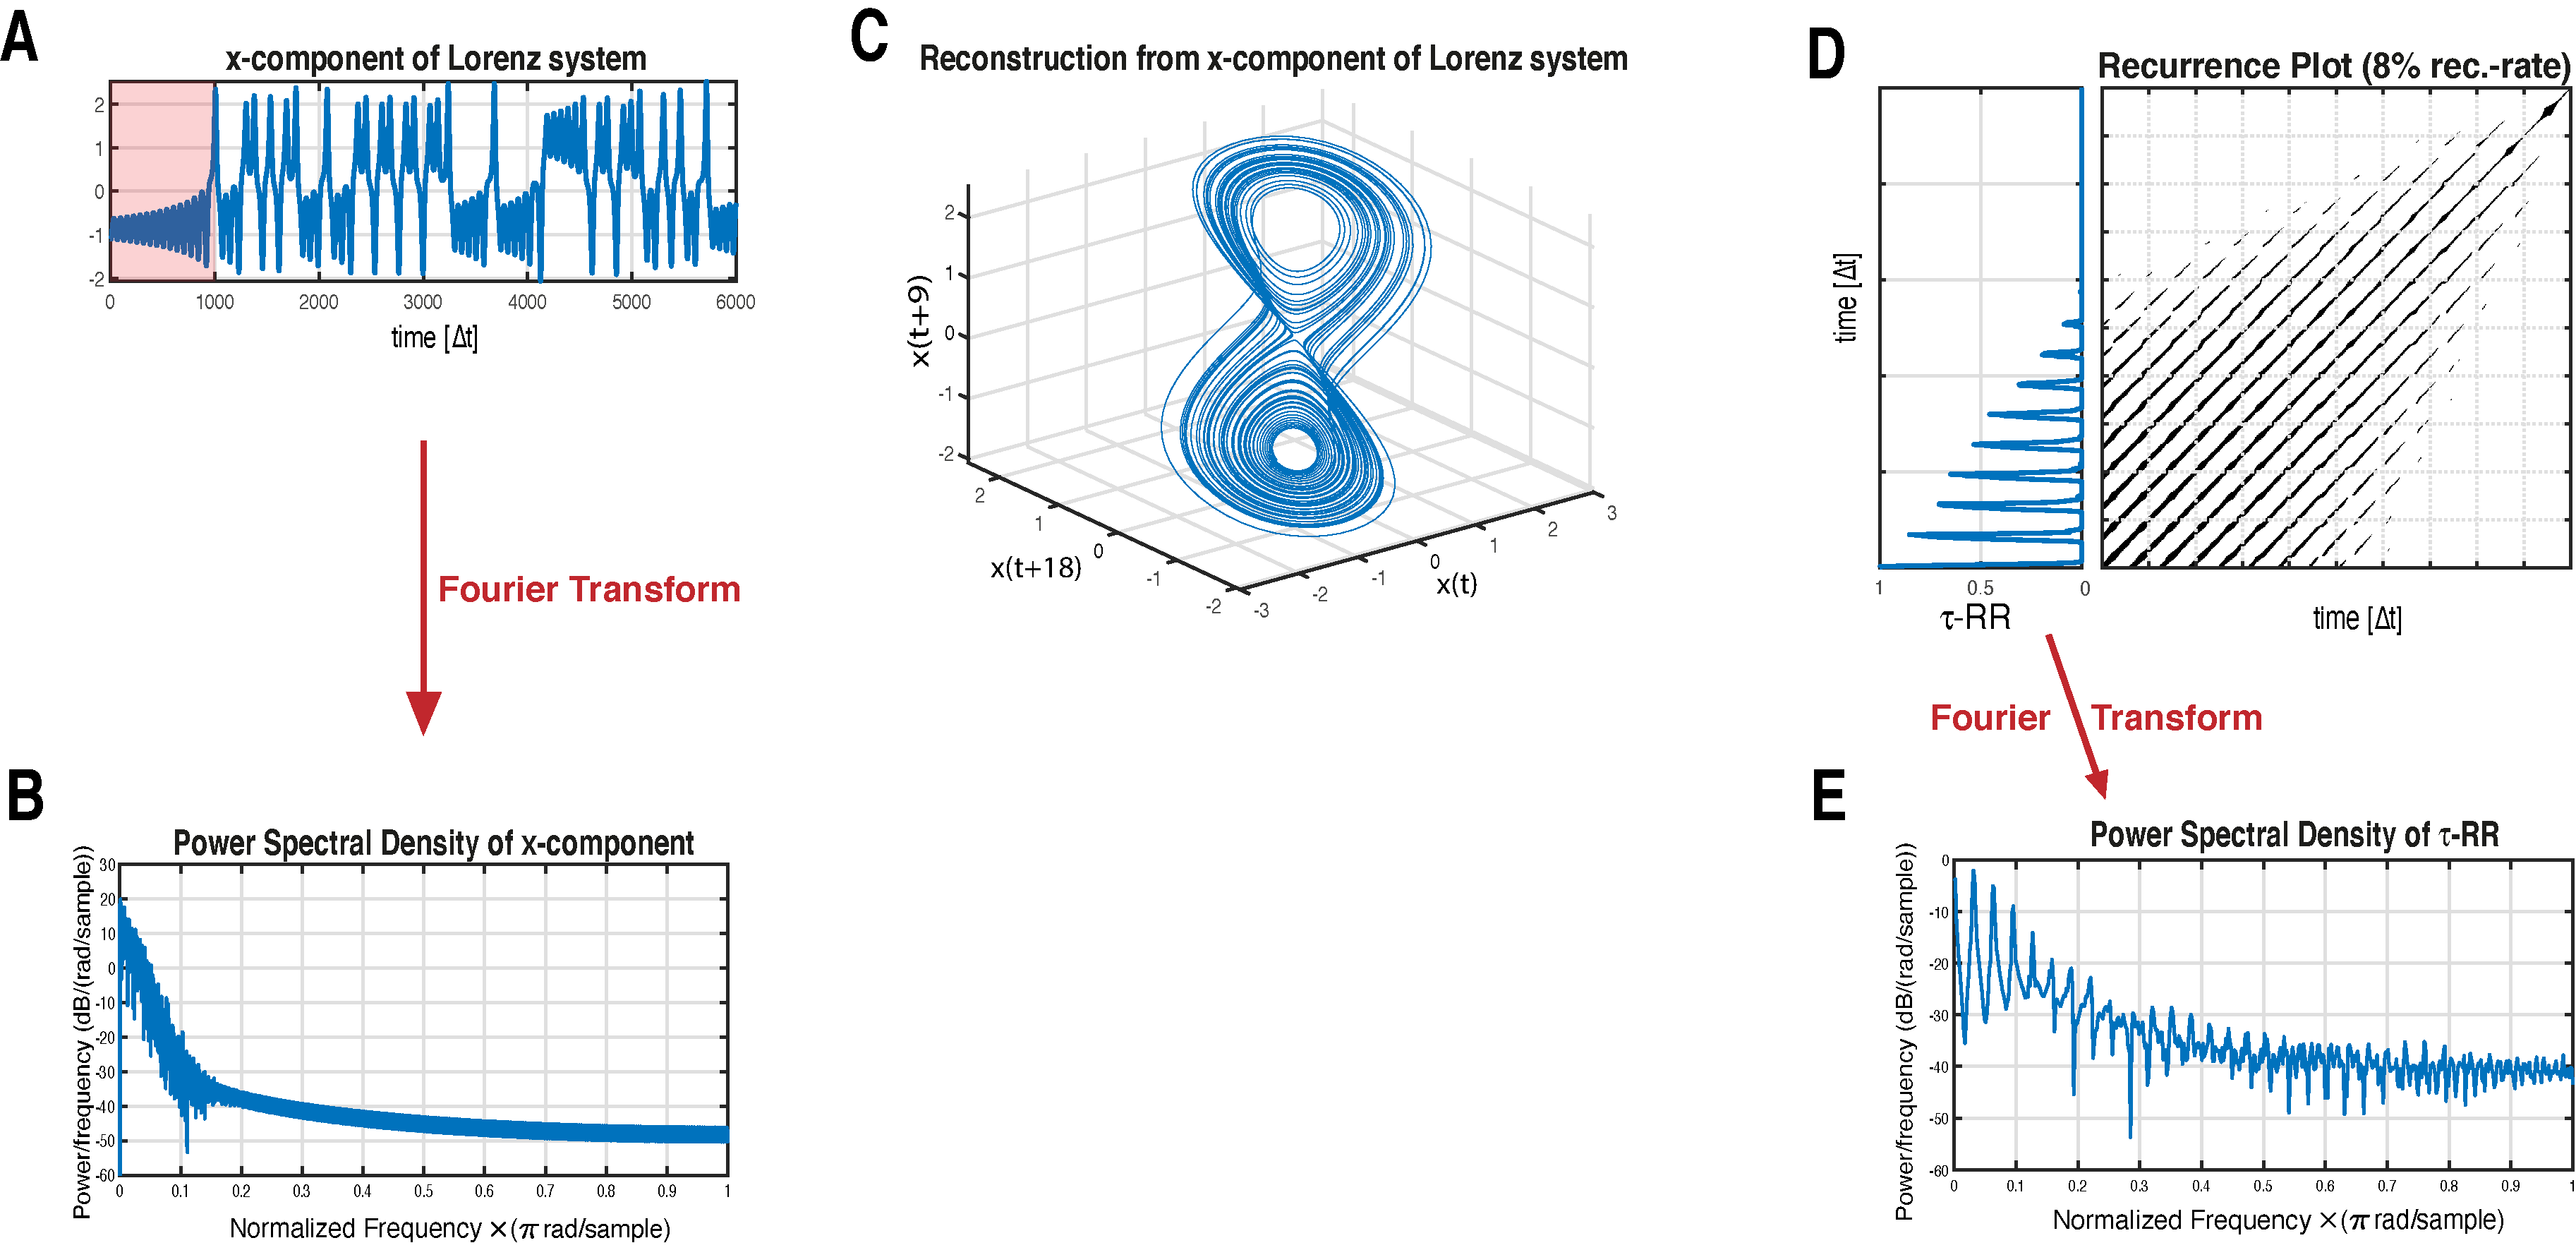
\includegraphics[width=0.9\textwidth]{./figures/fig_tau_rr_spectrum_example}
 \caption{Schematic illustration of a $\tau$-recurrence rate based spectrum. \textbf{A} $x$-component time series of the Lorenz63-System (Eq.~\eqref{eq_model_Lorenz63}) and 
 \textbf{B} its corresponding Fourier power spectrum. 
 \textbf{C} Reconstructed state space portrait from the time series shown in \textbf{A} using PECUZAL time-delay embedding \cite{Kraemer2021}. 
 \textbf{D} Subset of the recurrence plot and the corresponding $\tau$-recurrence rate obtained from the state space trajectory in \textbf{C}. 
 \textbf{E} Fourier Power spectrum obtained from the $\tau$-recurrence rate (subset shown in panel \textbf{D}) \cite{Zbilut2008}. \textbf{D} and \textbf{E} show the results of a part of the time series, 
 which is highlighted in pink in \textbf{A}.
 }\label{fig_tau_rr_spectrum_example}
\end{figure}

However, the interpretation of this generalized power spectral density is unclear, and it is typically hard to interpret. $\tau$-RR directly encodes the periodicity of the underlying signal, in contrast it is unclear what, if any, interpretation the "power" contained in a particular frequency mode of the $\tau$-RR should have. Whenever $\tau$-RR is a spike-train-like signal, which it is in most cases (see Fig.~\ref{fig_tau_rr_spectrum_example}) especially for 
map-data (low-resolution data), a FT of such a signal leads to a spike-train-like image in the frequency domain (e.g., \cite{Schild1982,Cordoba1989}, see 
Fig.~\ref{fig_tau_rr_spectrum_example}E). Thus, it is not intuitive how to extract meaningful information about the systems' state space trajectory. 

For example, consider the signal we would like to analyze 
(e.g., the $\tau$-RR of a system) to be a Dirac comb (DC) with inter-spike period $T_\text{is}$: 
\begin{equation}
\text{DC}_{\text{is}}(t) = \sum_{k=-\infty}^{\infty} \delta(t-kT_\text{is}),
\label{eq_dirac_comb}
\end{equation}
i.e., a series of Dirac delta functions for a period $T_\text{is}$. There is only one single period, $T_\text{is}$, in this signal (Fig.~\ref{fig_tau_rr_dirac_comb}A, D), so 
in principle we would strive for a single peak in the frequency domain of this signal at a frequency $f=1/T_\text{is}$. The Fourier spectrum does not meet this expectation 
and instead of a single frequency, there are many frequencies excited (Fig.~\ref{fig_tau_rr_dirac_comb}B, E). This is because the Fourier components add constructively 
for every frequency $1/T_\text{is}$ and therefore $\text{DC}_{\text{is}}(t)$ coincides with its own Fourier transform up to a factor $1/T_\text{is}$ \cite{Norden1998}.\footnote{This can also 
be observed for neuron spike trains, e.g. \cite{Orcioni2020,Biagetti2017}.}

\begin{figure}[h]
 \centering
 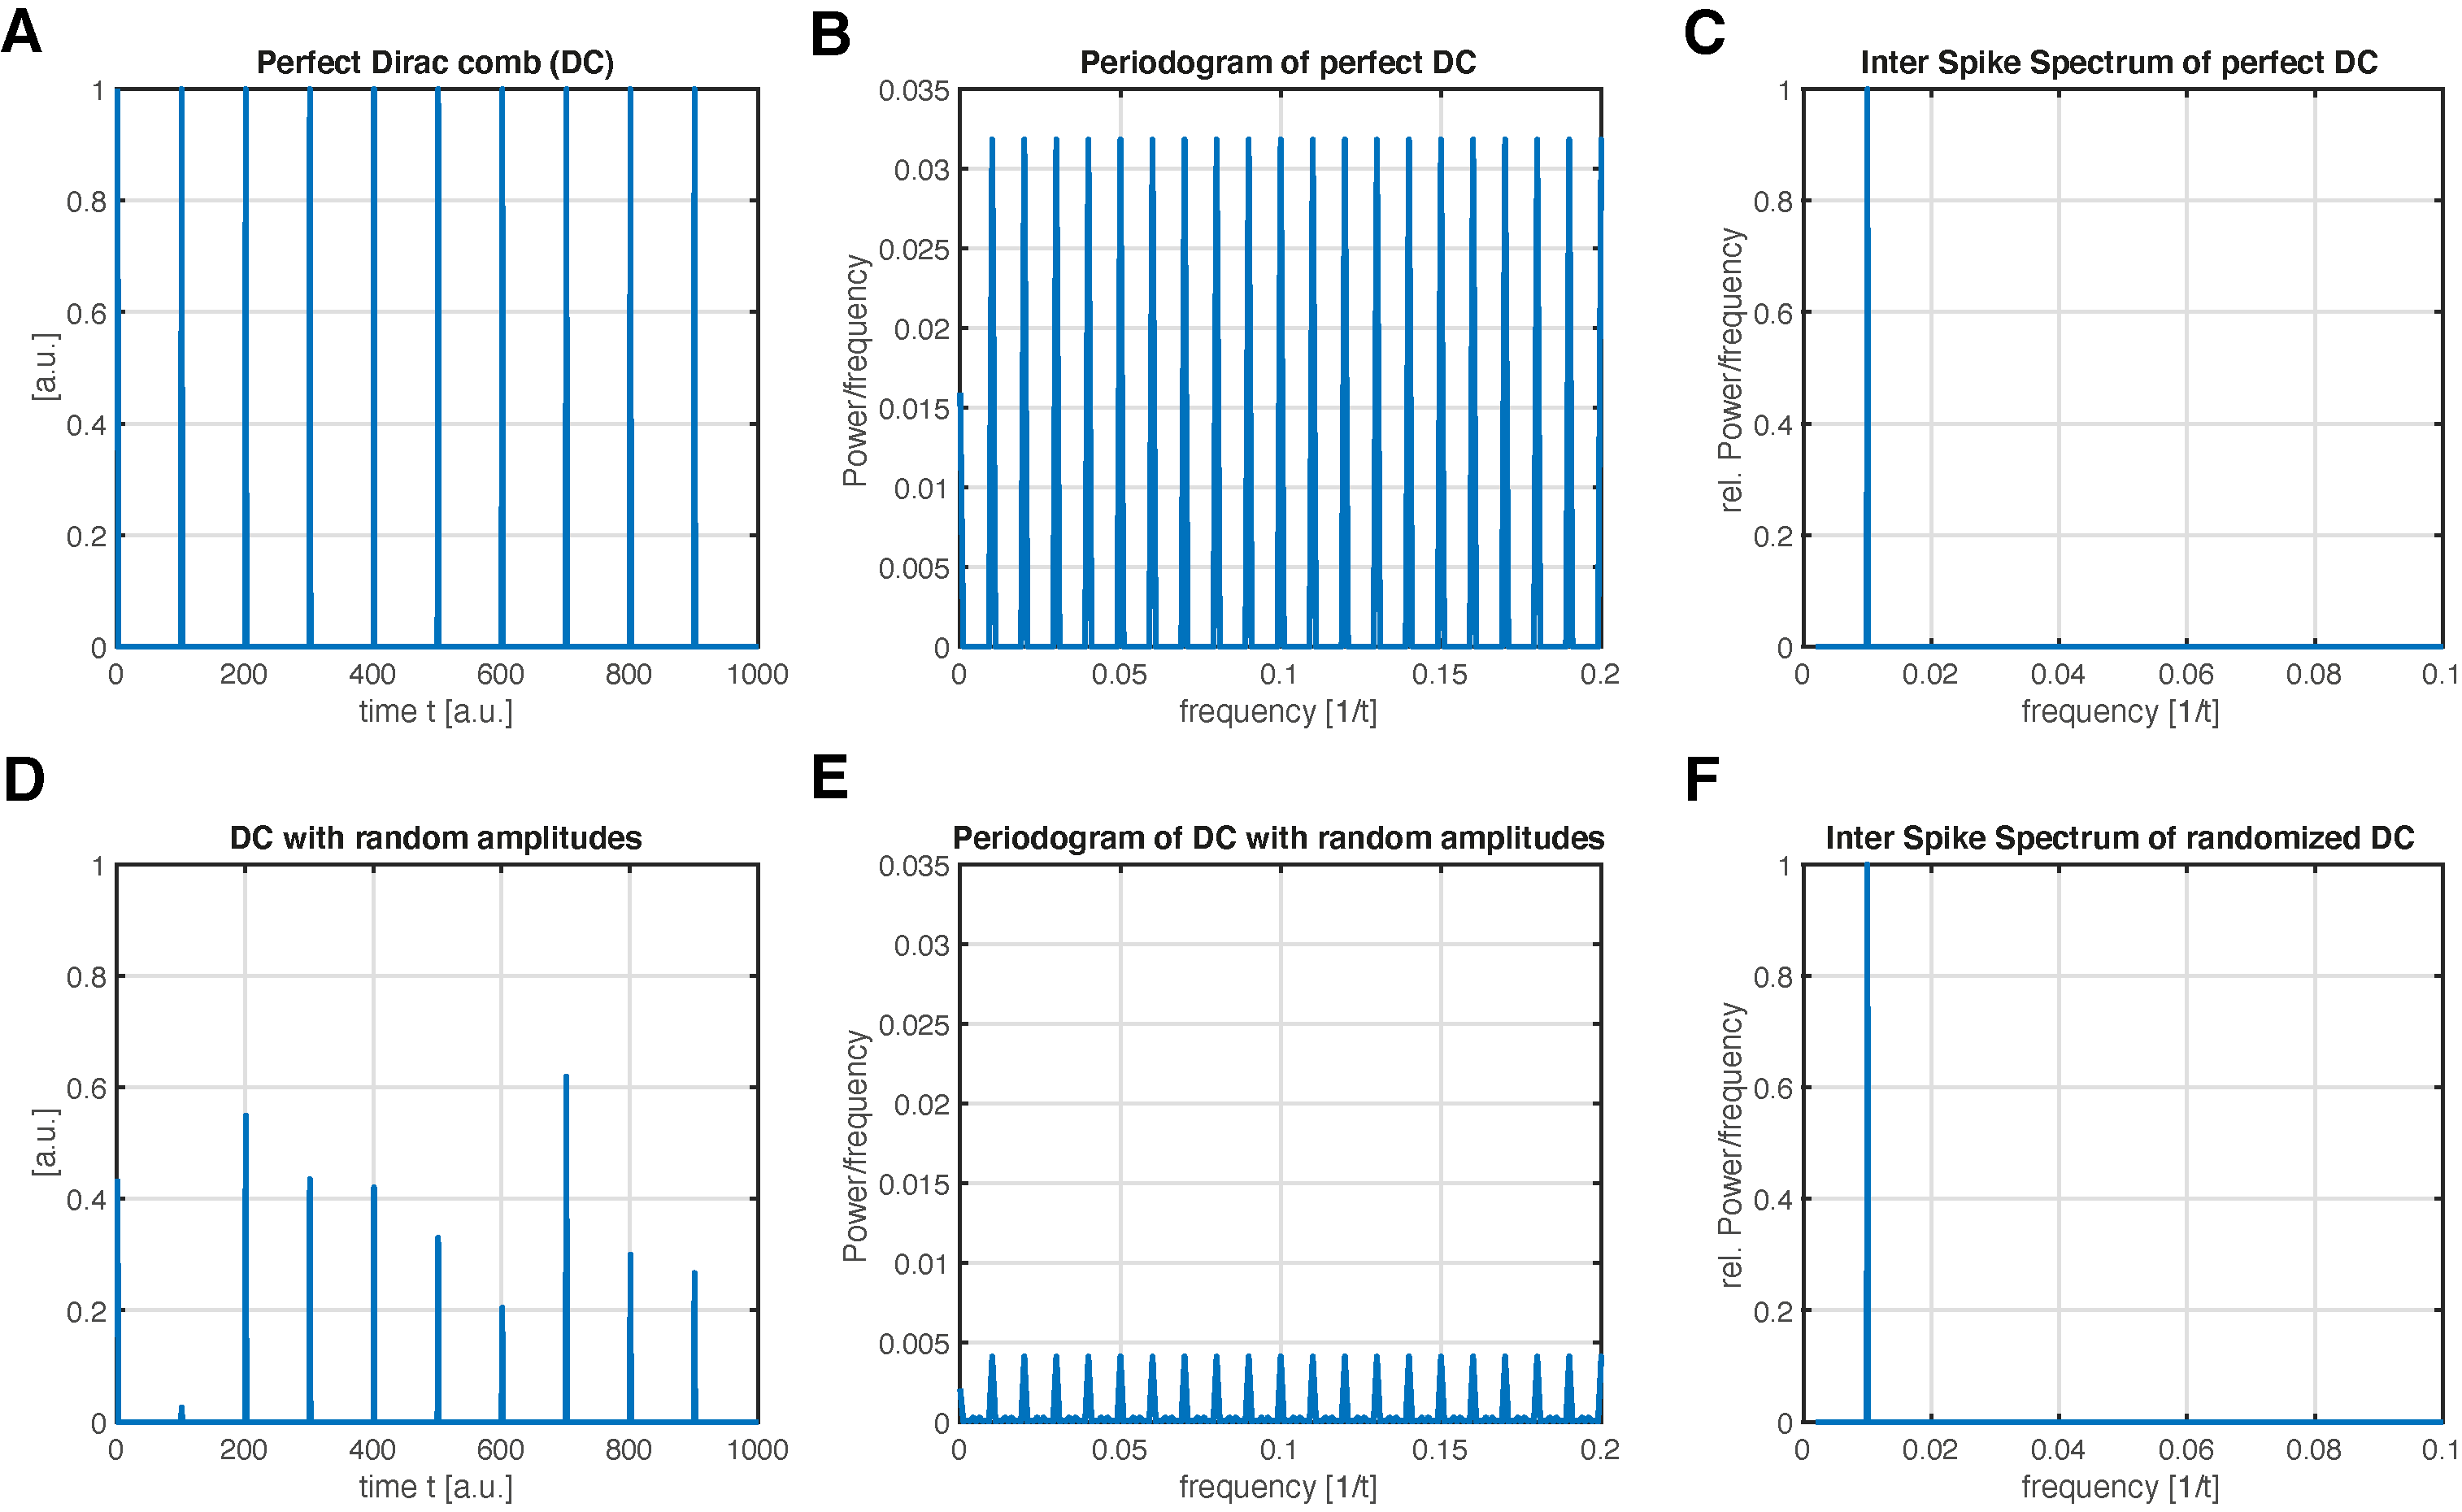
\includegraphics[width=0.9\textwidth]{./figures/fig_tau_rr_dirac_comb}
 \caption{The transformation of a Dirac comb (series of Dirac delta functions) with a single inter-spike period $T_{\text{is}}=100$ ($\widehat{=}f=0.01$) 
 into the frequency domain. 
 \textbf{A} Dirac Comb (DC) with equal amplitudes and
 \textbf{B} its FFT-based power spectral density.
 \textbf{C} Proposed inter-spike spectrum of the signal in \textbf{A} showing a single frequency, which corresponds to the inter-spike period $T_{\text{is}}$ ($f=0.01$).
 \textbf{D} DC with randomly chosen amplitudes and same $T_{\text{is}}$ as in \textbf{A}, and
 \textbf{E} its FFT-based power spectral density. 
 \textbf{F} Proposed inter-spike spectrum of the signal in \textbf{D} showing a single frequency, which corresponds to the expected inter-spike period $T_{\text{is}}$ ($f=0.01$). 
 Inter-spike spectra were obtained with a LASSO regression and a regularization threshold corresponding to $\rho=0.9$ accordance of the signals in (\textbf{A},\textbf{D}) and 
 its re-composed signals (c.f. Section~\ref{sec_tau_rr_method}). 
}
\label{fig_tau_rr_dirac_comb}
\end{figure}

In this article we propose a new way of decomposing a spike-train-like signal into periodic components as 
an alternative to the RP-based method suggested in \cite{Zbilut2008} or Fourier-based spike-train power 
spectra \cite{Dummer2014}. This novel \textit{inter-spike spectrum} does not show resonance 
behavior of the signal's inherent inter-spike frequencies in such a way that harmonics of these frequencies are also excited (Fig.~\ref{fig_tau_rr_dirac_comb}C, F). Section \ref{sec_tau_rr_method} explains the idea. Note that this approach can be used to decompose arbitrary signals, and is not specific to $\tau$-RR. However, the more spiky the signal is, the more useful our new approach is compared to a 
FT. In Section \ref{sec_tau_rr_application} we demonstrate the usage of inter-spike spectrum when transforming the $\tau$-RR of a system under study. In this case, the inter-spike spectrum 
can unravel characteristic time scales of high dimensional systems, which is not possible when using a FT. Finally, in Section \ref{sec_tau_rr_conclusion} our results are summarized.


%%%%%%%%%%%%%%%%%%%%%%%%%%%%%%%%%%%%%%%%%%
\section{Method}\label{sec_tau_rr_method}
    

To obtain the inter-spike spectrum, the signal, which we would like to analyse, in our case the $\tau$-RR, is decomposed into a set of appropriate basis functions. 
The general idea common to many methods is that the sum of these weighted functions can approximate a finite signal to a sufficient degree. The weights (in some contexts also called modes or loadings) corresponding to the individual basis functions must be determined.
A number of decomposition techniques based on different sets of basis functions exist, e.g., 
trigonometric functions (Fourier- and wavelet analysis \cite{Bracewell1986}), 
eigenvectors of the corresponding covariance matrix (principal component analysis \cite{Hotelling1933} and related techniques) 
or intrinsic mode functions (empirical mode decomposition and Hilbert spectrum \cite{Norden1998}).
These methods typically share the property that the basis functions form a complete basis,
the set of basis functions is linearly independent, and, thus, the weights are uniquely determined.

Here we propose to use Dirac combs (DC) with 
different inter-spike periods as basis functions, Eq.~\eqref{eq_dirac_comb}. Let $s(t_i)$ be the min-max-normalized signal we want to transform of length $N$ and 
$t_i=i\cdot \Delta t,~i=1,\ldots,N$, where $\Delta t$ denotes the sampling time and $s(t_i) \in [0,\ 1]\ \forall\ i$. In the following we label this time series as a $(1\times N)$-dimensional 
vector $\vec{s}$. 
First, $\tilde{N}$ different DCs of length $N$ are constructed with inter-spike periods $T_\text{is} \in [1,\ldots,\tilde{N}]$ and $\tilde{N}=\ceil*{N/2}+1$. Second, in order to account 
for possible phase shifts of 
these basis functions occurring in $\vec{s}$, each of these $\tilde{N}$ different DCs also need to be shifted one step further $T_\text{is}-1$ times. This leaves us with a total number of 
$M = \sum_{i=1}^{\tilde{N}}i$ 
\todo[inline]{let's come back to your example in Fig.~\ref{fig_tau_rr_basis_functions}, where $N=4$, regarding your explanation $M=\Sigma_i^{\tilde{N}=3} i= 1+2+3=6$. So finally matrix X should be 6x4 size. However, X does not have this size in Fig.3, which is the source of confusion.}
basis functions which we can arrange as rows of a $(M\times N)$-sized matrix $\bfX$
(Fig.~\ref{fig_tau_rr_basis_functions} illustrates the described procedure) \todo[inline]{(Moreover, although you claim above that number of rows in X is M in eq. (5) you say $\tilde{N}$, and in Fig. 3 it is four. You should really make it clear and cons)}:
\begin{align}
\label{eq_basis_matrix} 
\bfX_{i,j} &= \sum_{k=0}^{N}\delta\bigl(j-1-kT_\text{is}(i)-i+T_\text{is}(i) \bigr), \quad i=1,\dots,\ceil*{N/2}+1, \quad j=1,\dots,N\\
\label{eq_T_is} T_\text{is}(i)&= n, \quad \text{such that}\quad n:~ \frac{n(n-1)}{2} + 1 \leq i <  \frac{n(n+1)}{2} + 1,\quad n \in \mathbb{N}_+.
\end{align}

Note that due to the shifting of each of the basis functions of inter-spike period $T_\text{is}$, $\bfX$ is not linear independent anymore. 
Furthermore, there will be identical basis functions and also basis functions, which do not allow for an unambiguous inter-spike period, 
if we would include all $N$ possible inter-spike periods for a signal of length $N$ instead of $\ceil*{N/2}+1$ (Fig.~\ref{fig_tau_rr_basis_functions}A).
The reason is that in contrast to a trigonometric decomposition, where the Nyquist frequency marks a lower bound for the corresponding wave period, here 
the maximum considered inter-spike period is bounded by $T_{\text{is}}^{\text{max}} = \ceil*{N/2}+1$ (schematically illustrated in 
Fig.~\ref{fig_tau_rr_basis_functions}B). 

Eventually, an under-determined linear system
\begin{equation}
\bfX^T \boldsymbol{\beta}=\vec{s}
\label{eq_linear_system}
\end{equation}  
has to be solved for $\boldsymbol\beta$, a $(M\times 1)$-sized vector carrying the loadings we are interested in. Along a variety of algorithms which can solve this problem, we are 
particularly interested in those solutions, which promote sparsity in $\boldsymbol\beta$, since our goal is to decompose the signal $\vec{s}$ into a minimal number of basis 
functions (for an excellent overview of the topic we refer to \citet{Brunton2019}). In this paper we either use the \textit{least absolute shrinkage and selection operator} 
(LASSO) \cite{Tibshirani1996} or a \textit{sequentially thresholded least squares} (STLS) regression \cite{Brunton2016,Brunton2019} to obtain a solution $\hat{\boldsymbol\beta}$. Any other 
sparse regression technique could be used. Finally, we group loadings 
which correspond to basis functions having the same period 
$T_\text{is}$ into $\hat{\boldsymbol\beta}_f$ and obtain the 
\textit{inter-spike spectrum} by simply plotting $\hat{\boldsymbol\beta}_f$ as a function of the frequency $f=T_\text{is}^{-1}$, with $T_\text{is}=\Delta t, 2\Delta t, \dots, (\ceil*{N/2}+1) \Delta t$ 
(Fig.~\ref{fig_tau_rr_dirac_comb}C, F).

\begin{figure}
\centering
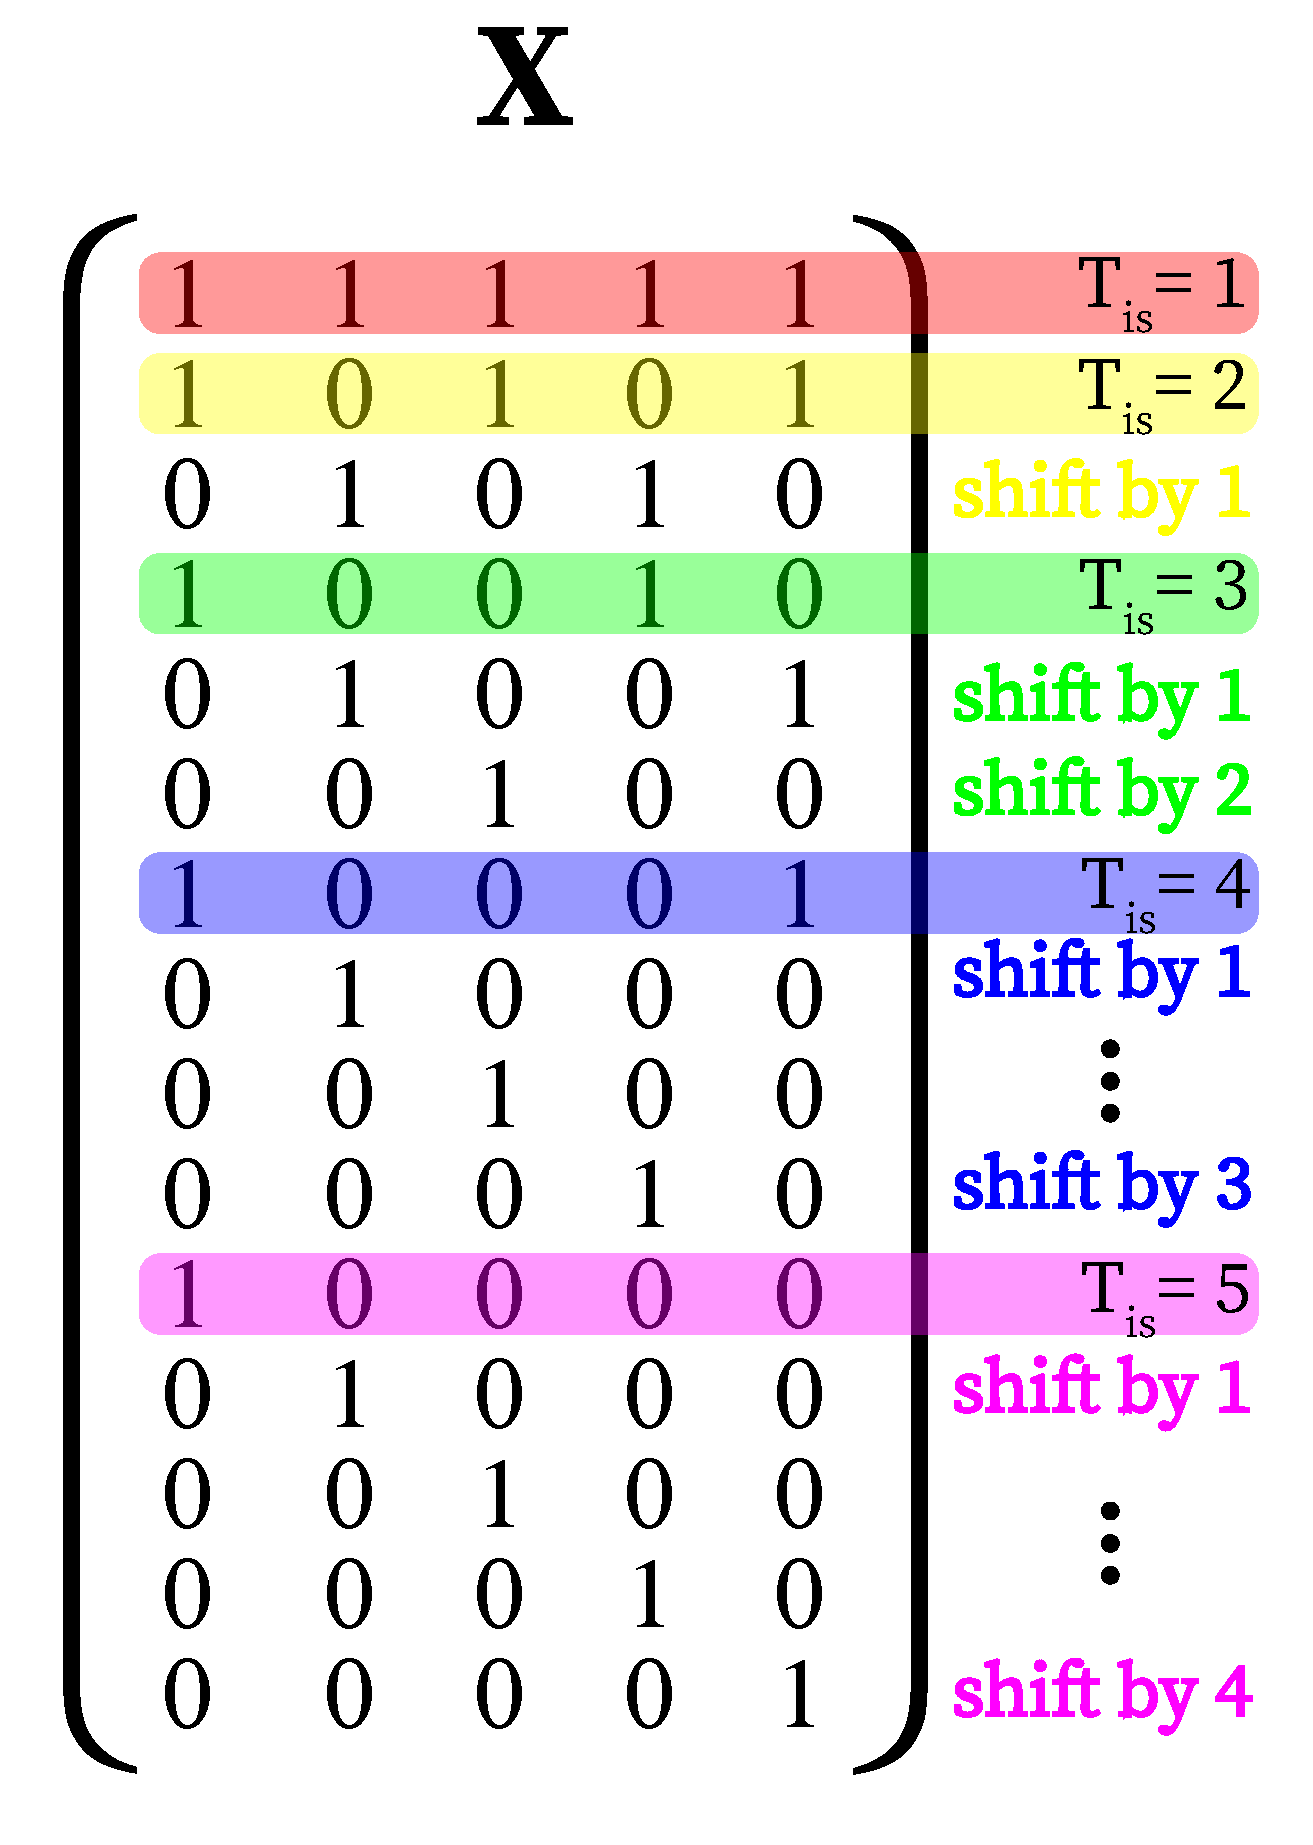
\includegraphics[width=0.9\textwidth]{./figures/fig_tau_rr_basis_functions}
\caption{\textbf{A} Example for a full set of basis functions for an input signal of length $N=4$, aligned in the matrix $\bfX'$. inter-spike periods $T_{\text{is}}$ larger 
than $\ceil*{N/2}+1$ lead to redundant basis functions (i.e., repeated lines in $\bfX$, red sheared) or basis functions, which cannot be uniquely assigned to a certain inter-spike period 
(blue sheared). $T_{\text{is}}$ for each row can be obtained by Eq.~\eqref{eq_T_is}. \textbf{B} The final set of unambiguous, but still linearly dependent, basis functions aligned in the matrix $\bfX$.} \label{fig_tau_rr_basis_functions}
\end{figure}

<<<<<<< HEAD
When introducing a sparsity regularization we give up the ability to fully reconstruct the signal from the decomposition in favor of identifying the most prominent spikes, and, thus, the most important periodicities more clearly. This choice is parametrized by a regression regularization parameter $\alpha$. Only for $\alpha = 0$ do we obtain a solution to Eq.~(\ref{eq_linear_system}) and, thus, a full reconstruction of the signal. Our general approach to fixing $\alpha$ is to require that we preserve most of the original signal in the sense of matching a given (Pearson) correlation coefficient $\rho$ between the original signal $\vec{s}$ and the reconstruction. The chosen regression method (in our case, LASSO or STLS) will determine how sensitive the obtained inter-spike spectrum is with respect to the regularization given by a 
selected $\rho$ (Fig.~\ref{fig_regularization} {\color{red}(It should not be Fig. A3? or you are talking about regularization parameter $\alpha$?)}). Regarding this, in most of our applications LASSO yields more robust results, while STLS is usually faster to compute. 
We will discuss this in more detail Section \ref{sec_tau_rr_discussion}.
=======
The proposed decomposition does not show a leakage effect by construction. However, when introducing a sparsity regularization we give up the ability to fully reconstruct the signal from the decomposition in favor of identifying the most important periodicities more clearly. This choice is mediated by a regression regularization parameter $\alpha$. Only for $\alpha = 0$ do we obtain a solution to Eq.~(\ref{eq_linear_system}) and thus a full reconstruction of the signal. Our general approach to fixing $\alpha$ is to require that we preserve most of the original signal in the sense of matching a given (Pearson) correlation coefficient $\rho$ between the original signal $\vec{s}$ and the reconstruction. The chosen regression method (in our case, LASSO or STLS) will determine how sensitive the obtained inter-spike spectrum is with respect to the regularization given by a 
selected $\rho$ (Fig.~\ref{fig_regularization}). Regarding this, in most of our applications LASSO yields more robust results, while STLS is usually faster to compute. 
We will discuss this in more detail in Section 4. Section \ref{sec_tau_rr_discussion}.
>>>>>>> 59451b9d30f76879c5a95867398fb09d3be77193

%
%In addition to the computational complexity of solving Eq.~\eqref{eq_linear_system}, the solving algorithm must also deal with the free choice of the regression regularization parameter $\alpha$, 
%which determines the sparsity of the regression coefficient vector $\hat{\boldsymbol\beta}$. Obviously, there will be numerous peaks in the inter-spike spectrum of a given signal, when $\alpha$ is small, 
%since $\alpha=0$ corresponds to the least squares solution and the corresponding $\hat{\boldsymbol\beta}$ is an exact solution of Eq.~(\ref{eq_linear_system}) and not sparse. On the other hand, 
%only a sparse number of non-zero loadings in $\hat{\boldsymbol\beta}$, i.e., peaks in the inter-spike spectrum, are obtained when $\alpha$ is sufficiently large. 
%The actual implementation of the regularization depends on the regression method chosen (in our case, LASSO or STLS), and consequently a given value of $\alpha$ will generally result in 
%different sparse loading vectors $\hat{\boldsymbol\beta}$. Therefore, in this paper we select $\alpha$ such that the re-composed signal $\tilde{\vec{s}}=\bfX^T\hat{\boldsymbol\beta}$ matches a 
%given (Pearson) correlation coefficient $\rho$ between the original signal $\vec{s}$ and itself.

%%%%%%%%%%%%%%%%%%%%%%%%%%%%%%%%%%%%%%%%%%
\section{Results}\label{sec_tau_rr_application}

We demonstrate the use of the inter-spike spectrum in combination with the $\tau$-RR as outlined in 
Section \ref{sec_tau_rr_intro} on several interesting research questions. The procedure is the following:
\begin{itemize}[noitemsep]
\item[(1)] Compute a RP of the trajectory of the system, Eq.~\eqref{eq_rp_definition}. If only univariate data is available, perform a state space reconstruction for obtaining the trajectory first.
\item[(2)] Compute the $\tau$-RR of that RP, Eq.~\eqref{eq_tau_rr}.
\item[(3)] Transform the $\tau$-RR into the proposed inter-spike spectrum, see Section \ref{sec_tau_rr_method}.
\end{itemize}


%%%%%%%%%%%%%%%%%%%%%%%%%%%%%%%%%%%%%%%%%%
\subsection{Period estimation for different dynamics in the R\"ossler system}
First, we consider the R\"ossler system (Eq.~\eqref{eq_model_roessler} in Appendix \ref{sec_models_roessler}) 
in three different dynamical setups. We use the proposed inter-spike spectrum to
identify the type of dynamics.
We set the parameters $b=2$, $c=4$ and analyze period-2 limit cycle dynamics ($a=0.36$ in Fig.~\ref{fig_tau_rr_example_roessler}A, D, G, J), 
period-3 limit cycle dynamics ($a=0.41$ in Fig.~\ref{fig_tau_rr_example_roessler}B, E, H, K) and chaotic dynamics ($a=0.428$ in Fig.~\ref{fig_tau_rr_example_roessler}C, F, I, L).  

\begin{figure}
 \centering
 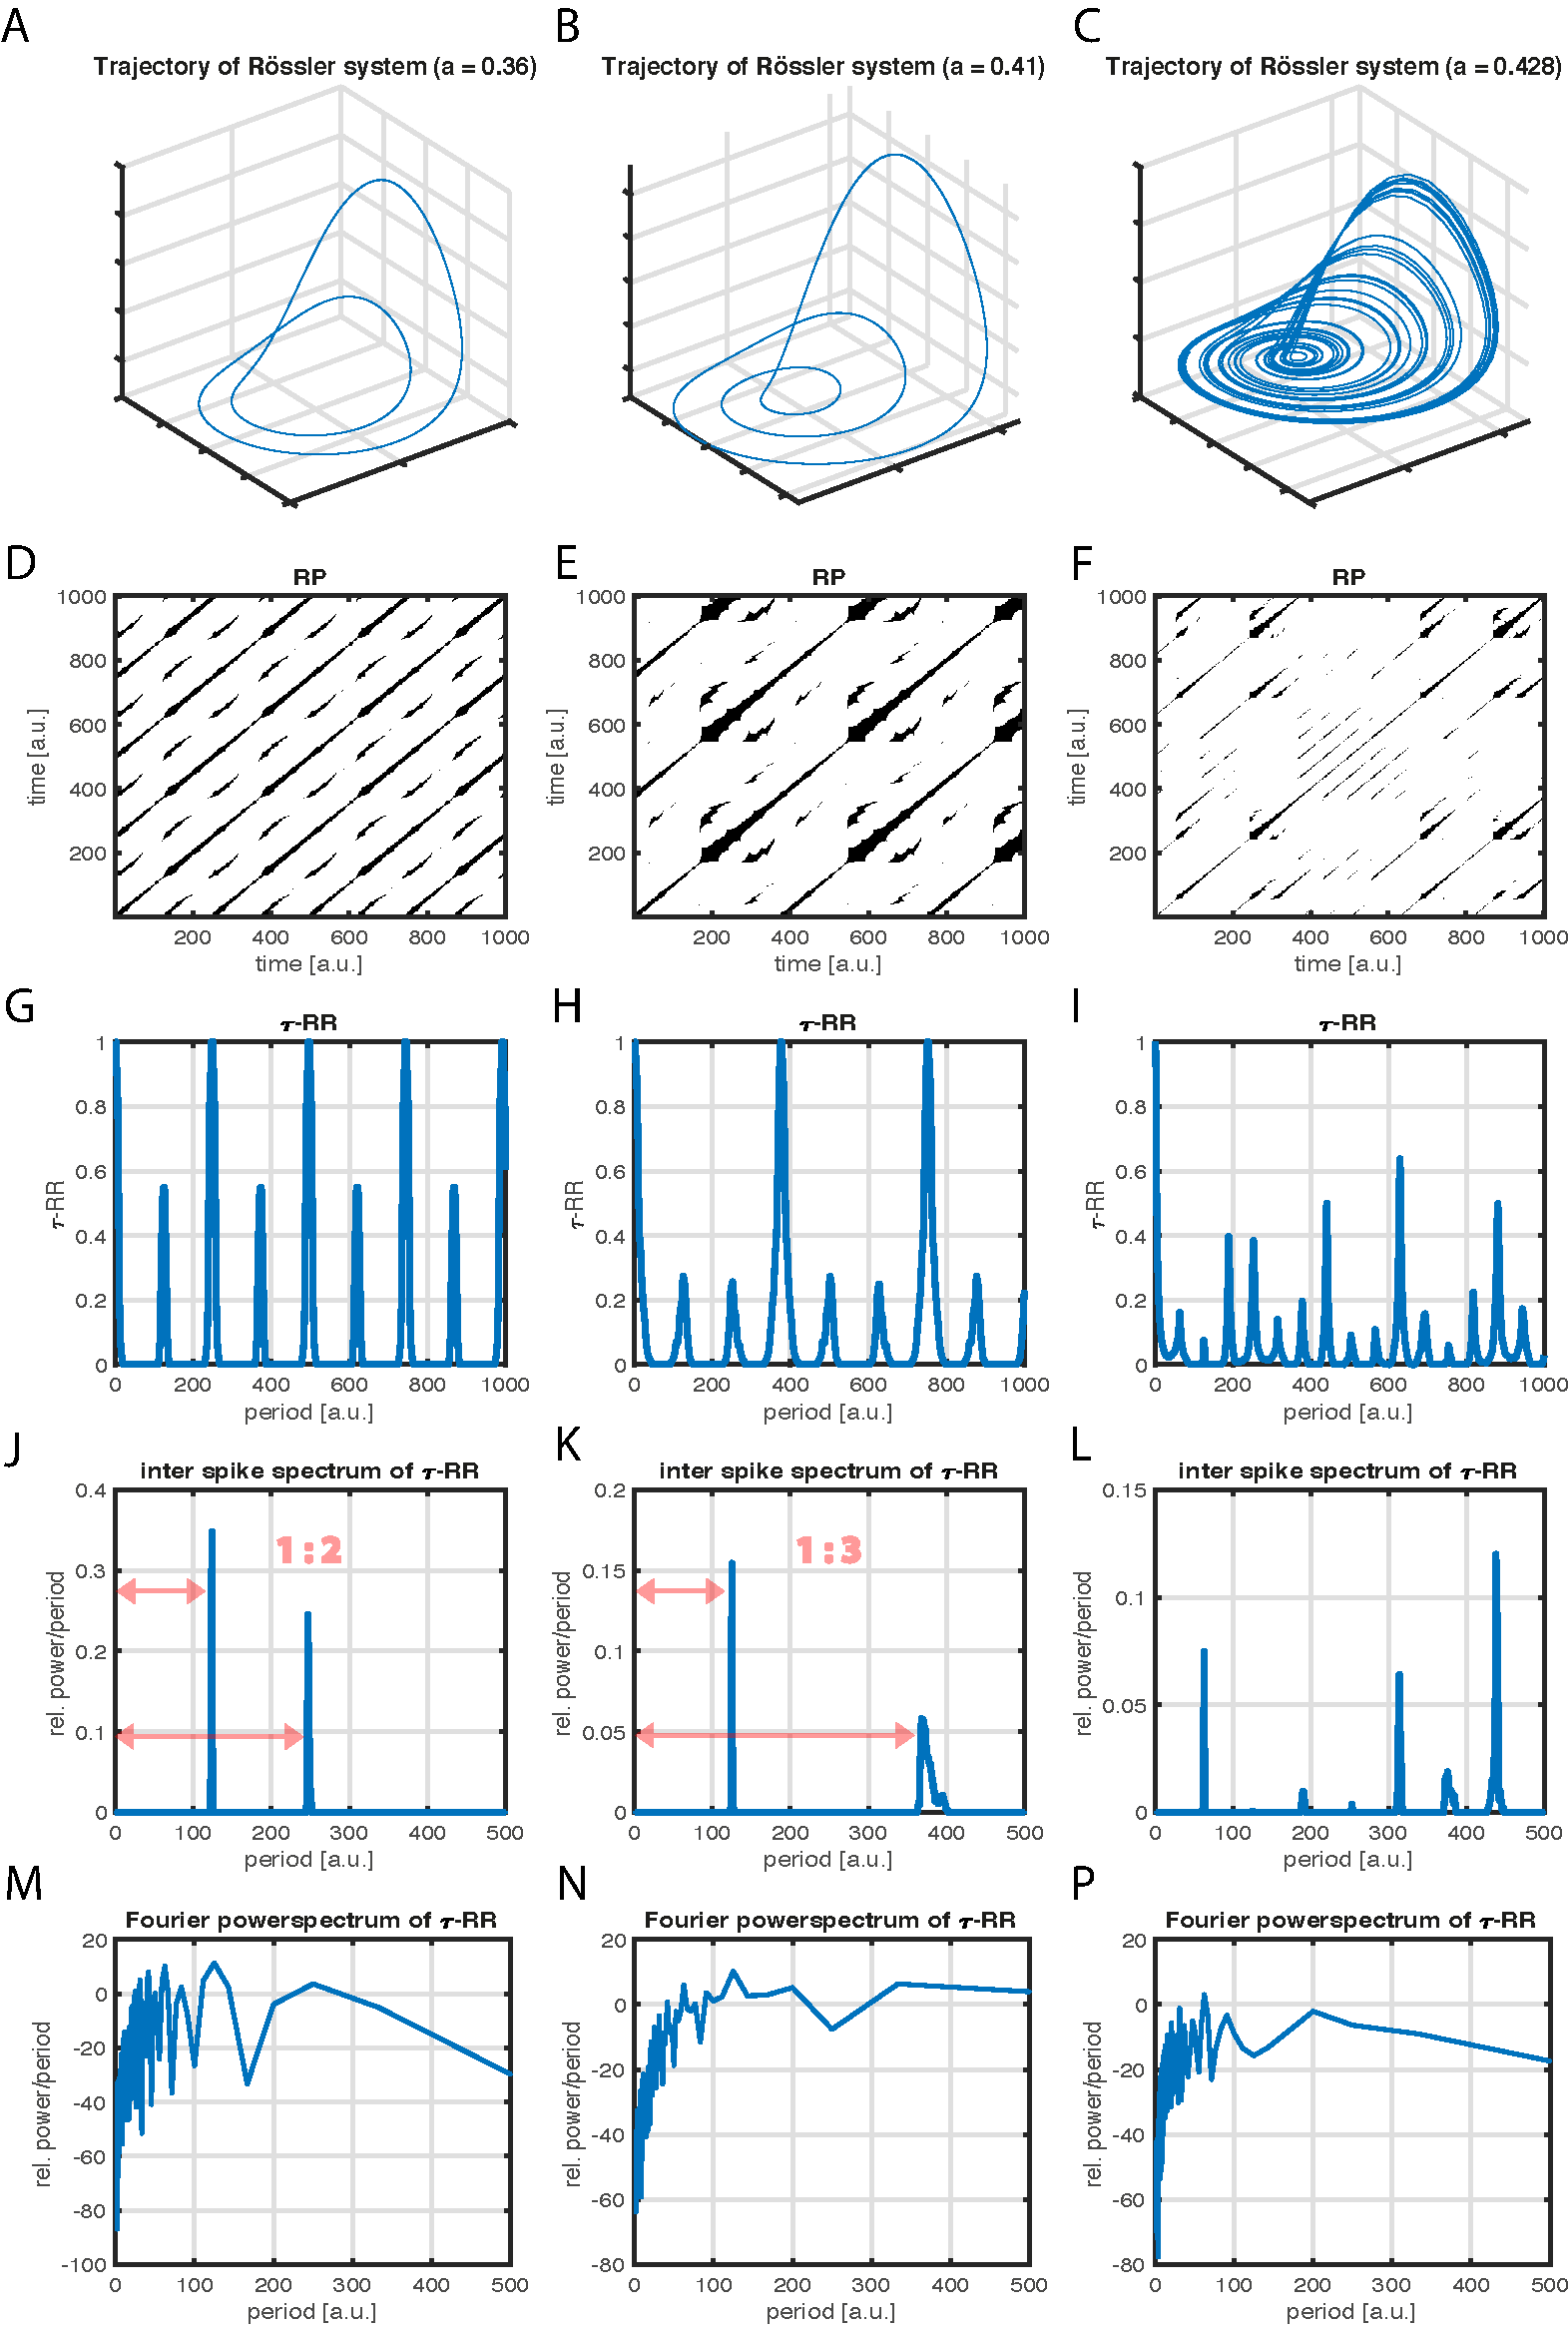
\includegraphics[width=0.9\textwidth]{./figures/fig_tau_rr_example_roessler}
 \caption{Inter-spike spectra of the $\tau$-RR of the R\"ossler system in three different dynamical regimes with parameters $b=2$, $c=4$. 
 \textbf{A} Trajectory of the system in a period-2 (parameter $a=0.36$), \textbf{B} in a period-3 (parameter $a=0.41$) and 
 \textbf{C} in a chaotic regime (parameter $a=0.428$). 
 \textbf{D, E, F} The corresponding RPs, obtained by using a recurrence threshold corresponding to a 10\% global 
 recurrence rate for D \& E and 5\% for F. 
  \textbf{G, H, I} $\tau$-RRs of the shown RPs. 
  \textbf{J, K, L} The proposed inter-spike spectra of the $\tau$-RRs shown in panels G, H, I. Spectra were obtained with a LASSO regression and a regularization threshold 
  corresponding to $\rho=0.95$ accordance of $\tau$-RRs and re-composed signals. The distance ratio of the peaks reflect the limit cycle dynamic.  
  \textbf{M, N, P} Fourier power spectra of the $\tau$-RRs shown in panels G, H, I. }
\label{fig_tau_rr_example_roessler}
\end{figure}

The inter-spike spectra unravel the specific dynamics, which are also apparent in the state space portraits (Fig.~\ref{fig_tau_rr_example_roessler}A, B, C) and in the 
$\tau$-RRs (Fig.~\ref{fig_tau_rr_example_roessler}G, H, I). The proposed idea is also 
robust to noise (see Fig.~\ref{fig_tau_rr_example_roessler_noise} in the Appendix). This is because the peaks of the $\tau$-RR are insensitive to noise. 
Figure \ref{fig_roessler_peaks} illustrates that 
while the peak shape does change in the presence of noise, its position does not, and this is what the inter-spike spectrum encrypts after all 
(see Fig.~\ref{fig_roessler_spectra_distances} in the Appendix for further analysis).

\begin{figure}
 \centering
 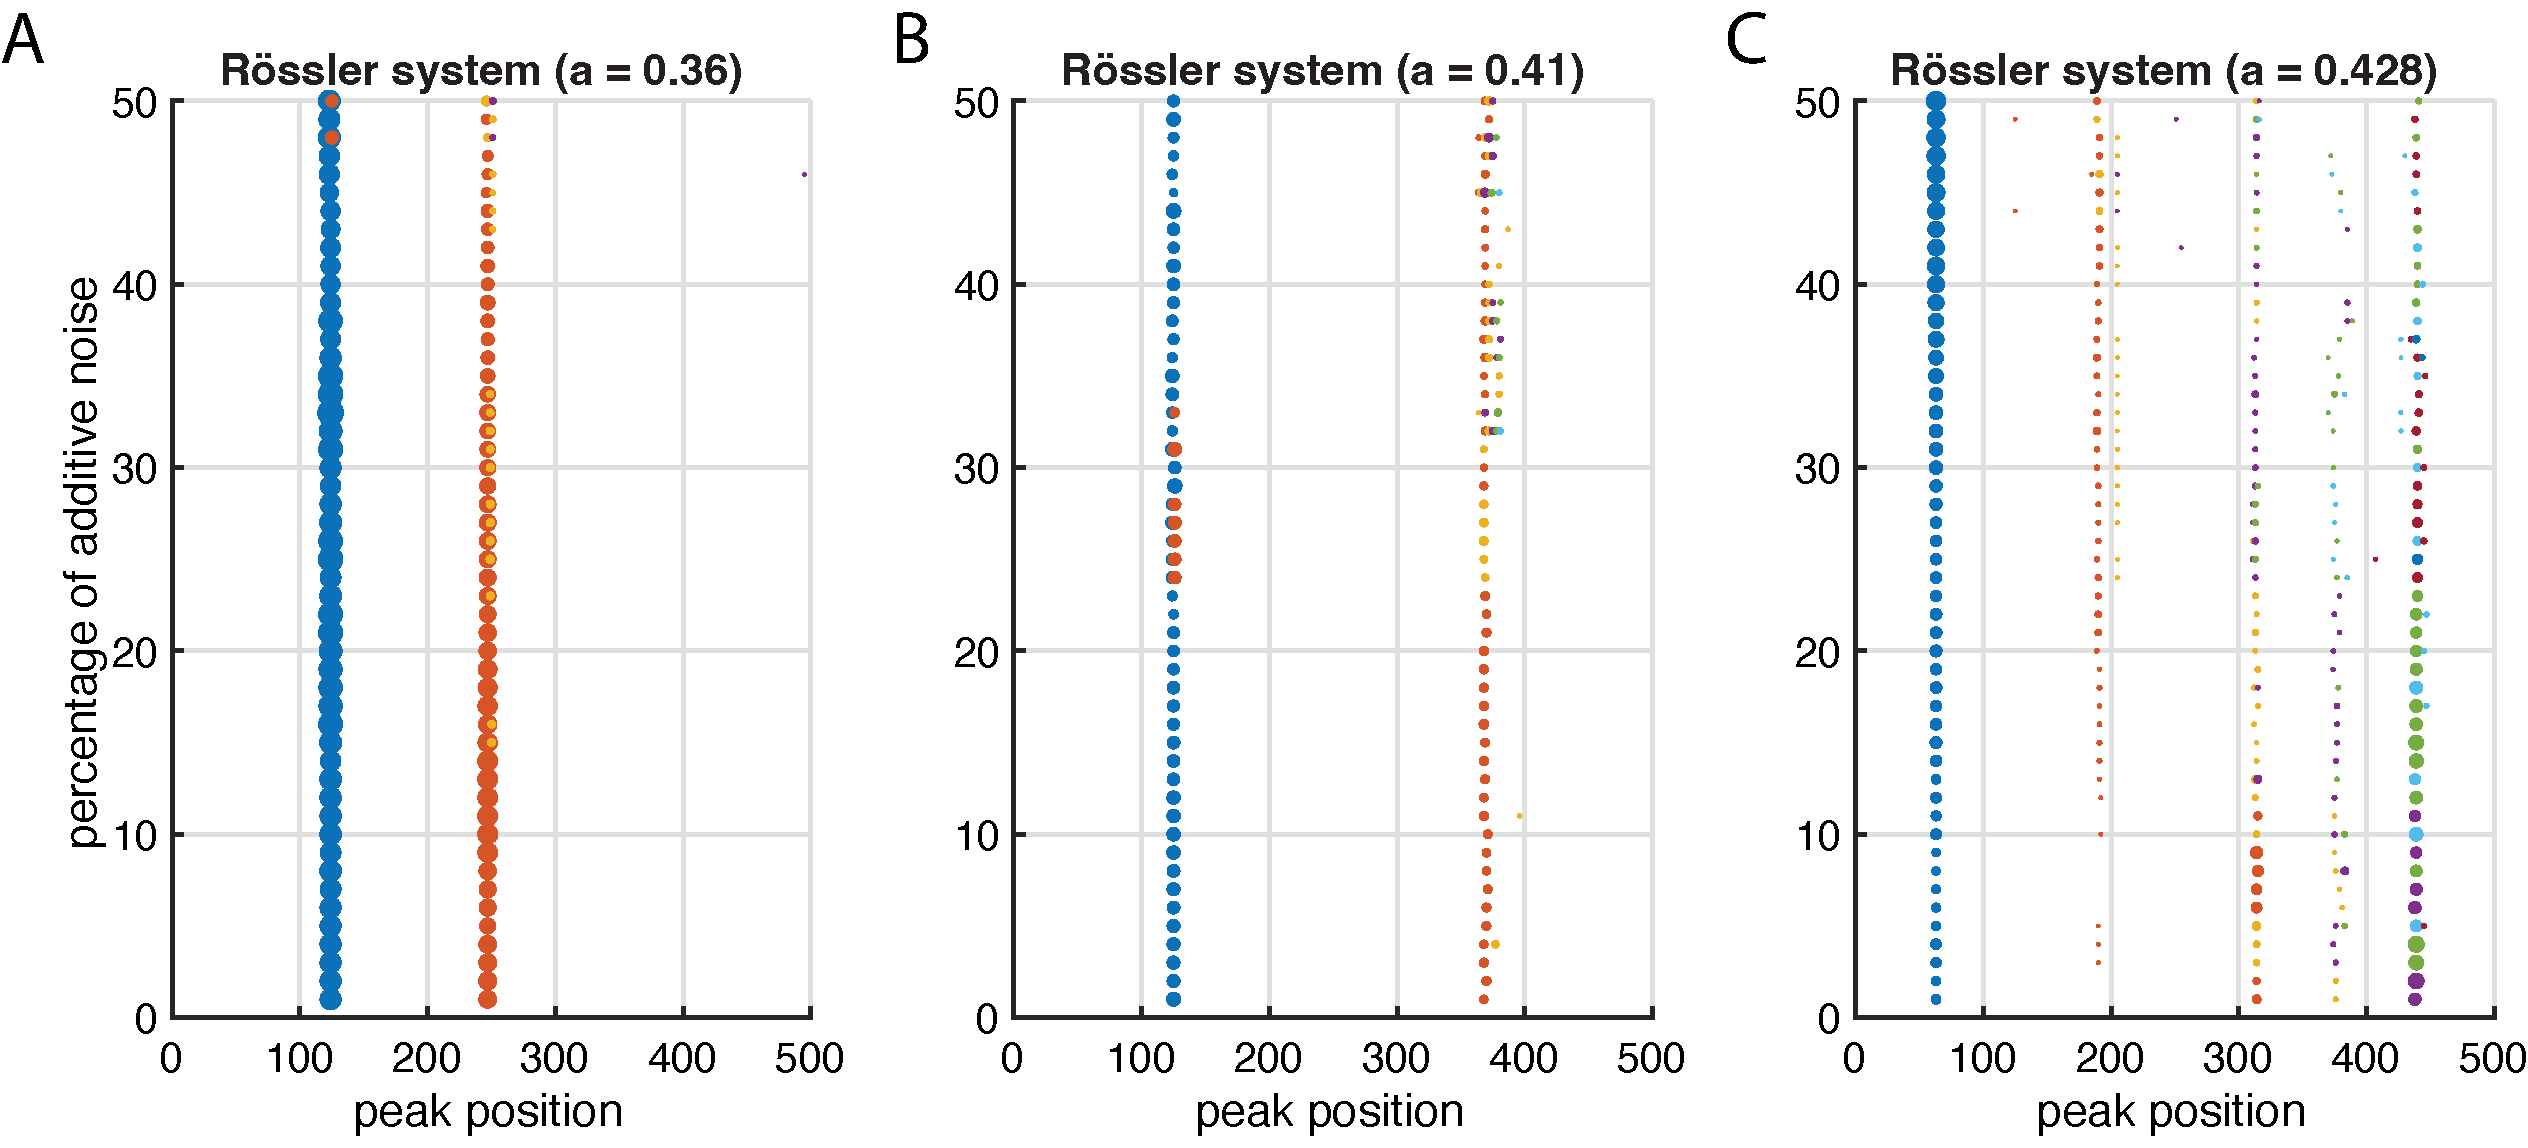
\includegraphics[width=0.9\textwidth]{./figures/fig_roessler_different_noise_levels_peaks}
 \caption{Peak positions of the obtained inter-spike spectra of the $\tau$-RRs for additive noise levels up to 50\% for the discussed R\"ossler dynamics, 
 \textbf{A} period-2 limit-cycle, \textbf{B} period-3 limit-cycle and \textbf{C} chaos. The size of the plotted markers scale with the detected peak height. The noise-free spectra are shown in Fig.~\ref{fig_tau_rr_example_roessler}J, K, L and 
 an example of these spectra with 5\% additive noise is shown in Fig.~\ref{fig_tau_rr_example_roessler_noise}J, K, L. Spectra were obtained with a LASSO regression and a regularization threshold 
  corresponding to $\rho=0.95$ accordance of $\tau$-RRs and re-composed signals.}
\label{fig_roessler_peaks}
\end{figure}


%%%%%%%%%%%%%%%%%%%%%%%%%%%%%%%%%%%%%%%%%%
\subsection{Bifurcations in the Logistic map}

We consider the Logistic map $x_{n+1}=r\cdot x_n \left( 1-x_n \right)$ for changing control parameter $r$. We vary $r$ from $r=3.4$ to $r=4$ in steps of $0.001$. For 
each setting of $r$ 
\begin{itemize}[noitemsep]
\item[(1)] a time series of length $N=201$ is computed with a random initial condition $u_0 \in [0,\ 1]$, neglecting the first $1,000$ samples as transients,
\item[(2)] $100$ iterative Amplitude Adjusted Fourier Transform (iAAFT) surrogates \cite{Schreiber1996,Schreiber2000} are computed,
\item[(3)] the time series and its iAAFT surrogates are embedded in a 2-dimensional state space using a time delay of unity,
\item[(4)] from the 2-dimensional trajectories RPs, Eq.~\eqref{eq_rp_definition}, are computed under a threshold $\varepsilon=0.05$,
\item[(5)] $\tau$-RR, Eq.~\eqref{eq_tau_rr}, is computed from the RP of the signal and from the RPs of the surrogates,
\item[(6)] inter-spike spectra are obtained from $\tau$-RR of the signal and from the $\tau$-RRs of the surrogates, see Section \ref{sec_tau_rr_method}, and finally,
\item[(7)] from the distribution of the surrogate inter-spike spectra the $95^\text{th}$ percentile is computed. The peaks of the inter-spike spectrum of the signal which exceed 
this percentile are counted. 
\end{itemize}
In this example, the according null hypothesis for constructing the surrogate data is that the data stems from a process which yields the same auto-correlation, 
hence, the same Fourier power spectral density, and the same 
amplitude distribution. We consider the number of significant peaks in the inter-spike spectrum with
respect to the control parameter in order to distinguish the corresponding dynamics (Fig.~\ref{fig_tau_rr_logistic}C).
A correlation with the positive Lyapunov exponent (Fig.~\ref{fig_tau_rr_logistic}A) is discernible 
($\rho_{\text{Pearson}}(\text{Lyapunov})=0.72$). This analysis can tackle period-doubling, since it ``measures'' the dominant cycles via the inter-spike spectrum. 
However, whenever the periods of the ``new'' cycles coincide with integer multiples of the periods of already existing cycles, this approach cannot detect 
period-doubling. A similar case can be observed in Fig.~\ref{fig_tau_rr_example_roessler}J,K where the number of peaks does not change, but  their mutual distance does. 

A less computationally intensive approach is to compute surrogates for the $\tau$-RR analytically, rather than computing a RP and its $\tau$-RR for each iAAFT surrogate of the 
time series. This translates into a null hypothesis 
that the $\tau$-RR and its corresponding inter-spike spectrum stems from a RP of a random signal. In this case the probability of finding a black point in the RP can be obtained 
from a binomial distribution with probability parameter $p$ set to the recurrence rate of the RP of the signal. This way $100$ surrogate $\tau$-RRs are computed in step (5). 
The results are even slightly better compared to the ones obtained from the iAAFT surrogates (Fig.~\ref{fig_tau_rr_logistic}B, $\rho_{\text{Pearson}}(\text{Lyapunov})=0.81$). 
The first period doubling at $r \approx 3.458$ cannot be detected by any of the surrogates.

The described procedure does work well for map data, because most often the $\tau$-RR for those kind of data reveals a ``spiky enough'' nature. 
On the contrary, highly sampled (flow-) data often yield not as 
spiky $\tau$-RRs and, thus, the number of significant peaks in the inter-spike spectrum may not be sensitive enough to detect period-doubling bifurcations. Moreover the sensitivity of the 
inter-spike spectrum to detect the regime shifts also depends on the critical regularization threshold. Nevertheless the 
according inter-spike spectra is still revealing important information (Fig.~\ref{fig_tau_rr_example_roessler}) and practitioners can design appropriate quantifying statistics based 
on these spectra, which suit the research task.

\begin{figure}
 \centering
 \includegraphics[width=\textwidth]{./figures/fig_tau_rr_logistic}
 \caption{\textbf{A} Bifurcation diagram and Lyapunov exponent and of the Logistic map as a function of the control parameter $r$.
 \textbf{B} Number of significant peaks ($\alpha=0.05$) in the inter-spike spectrum of the $\tau$-RR and its Pearson correlation coefficient to the Lyapunov exponent shown in \textbf{A} 
 (white noise surrogates). 
 \textbf{C} Same as \textbf{B}, but for iterative Amplitude Adjusted Fourier Transform (iAAFT) surrogates \cite{Schreiber1996,Schreiber2000}. For obtaining the inter-spike spectra we used 
 a LASSO regression and a regularization threshold corresponding to $\rho=0.95$ accordance of $\tau$-RRs and re-composed signals.  
}
\label{fig_tau_rr_logistic}
\end{figure}


%%%%%%%%%%%%%%%%%%%%%%%%%%%%%%%%%%%%%%%%%%
\subsection{inter-spike spectra of power grid frequency data}\label{sec_power_grid}

Power grids are large, synchronized, complex networks whose stable functioning is indispensable for modern societies.
To maintain the stability of a power grid, the balance between energy consumption and energy generation must be ensured. 
In an AC-power grid, the grid frequency is an observable variable that reflects how well this balance is satisfied. 
In this process, the grid frequency and its deviations from the nominal frequency are continuously recorded and monitored by 
the grid operators (in Europe and many parts of the world this is $50$ \si{Hz} or $60$ \si{Hz} in America and, for example, southern Japan).
For example, if there is more (less) demand than supply, the network frequency decreases (increases) compared to the nominal frequency \cite{kundur1994power}.


The frequency variations can include other information, such as the functionality of control systems \cite{gorjao2020data}, the effect of fluctuations in
renewable energies (REs), demands on the grid \cite{anvari2020stochastic} and, moreover, the effect of regular dispatches due to the trading market 
\cite{meyer2020identifying}. The latter induce periodic frequency jumps. Here we look at the frequency time series for the Great Britain (GB) and Continental Europe 
(CE) (Appendix \ref{sec_power_grid_appendix} and Fig.~\ref{fig_power_grid_time_series}A,C). Clear jumps every 30 and 60 minutes are discernible and quantitatively reflected in the corresponding 
autocorrelations (Fig.~\ref{fig_power_grid_time_series}B,D). Furthermore, the autocorrelation of the CE frequency time series shows regular peaks every $15$ \si{min} 
(see Fig.~\ref{fig_power_grid_time_series}B). These peaks are caused by a mismatch of power supply and demand \cite{weissbach2009high} during dispatches. 
In most electricity grids the operation of dispatchable power plants is scheduled in 1-hour blocks, where additional (shorter) $30$ and $15$ \si{min} intervals
might exist.


\begin{figure}
 \centering
 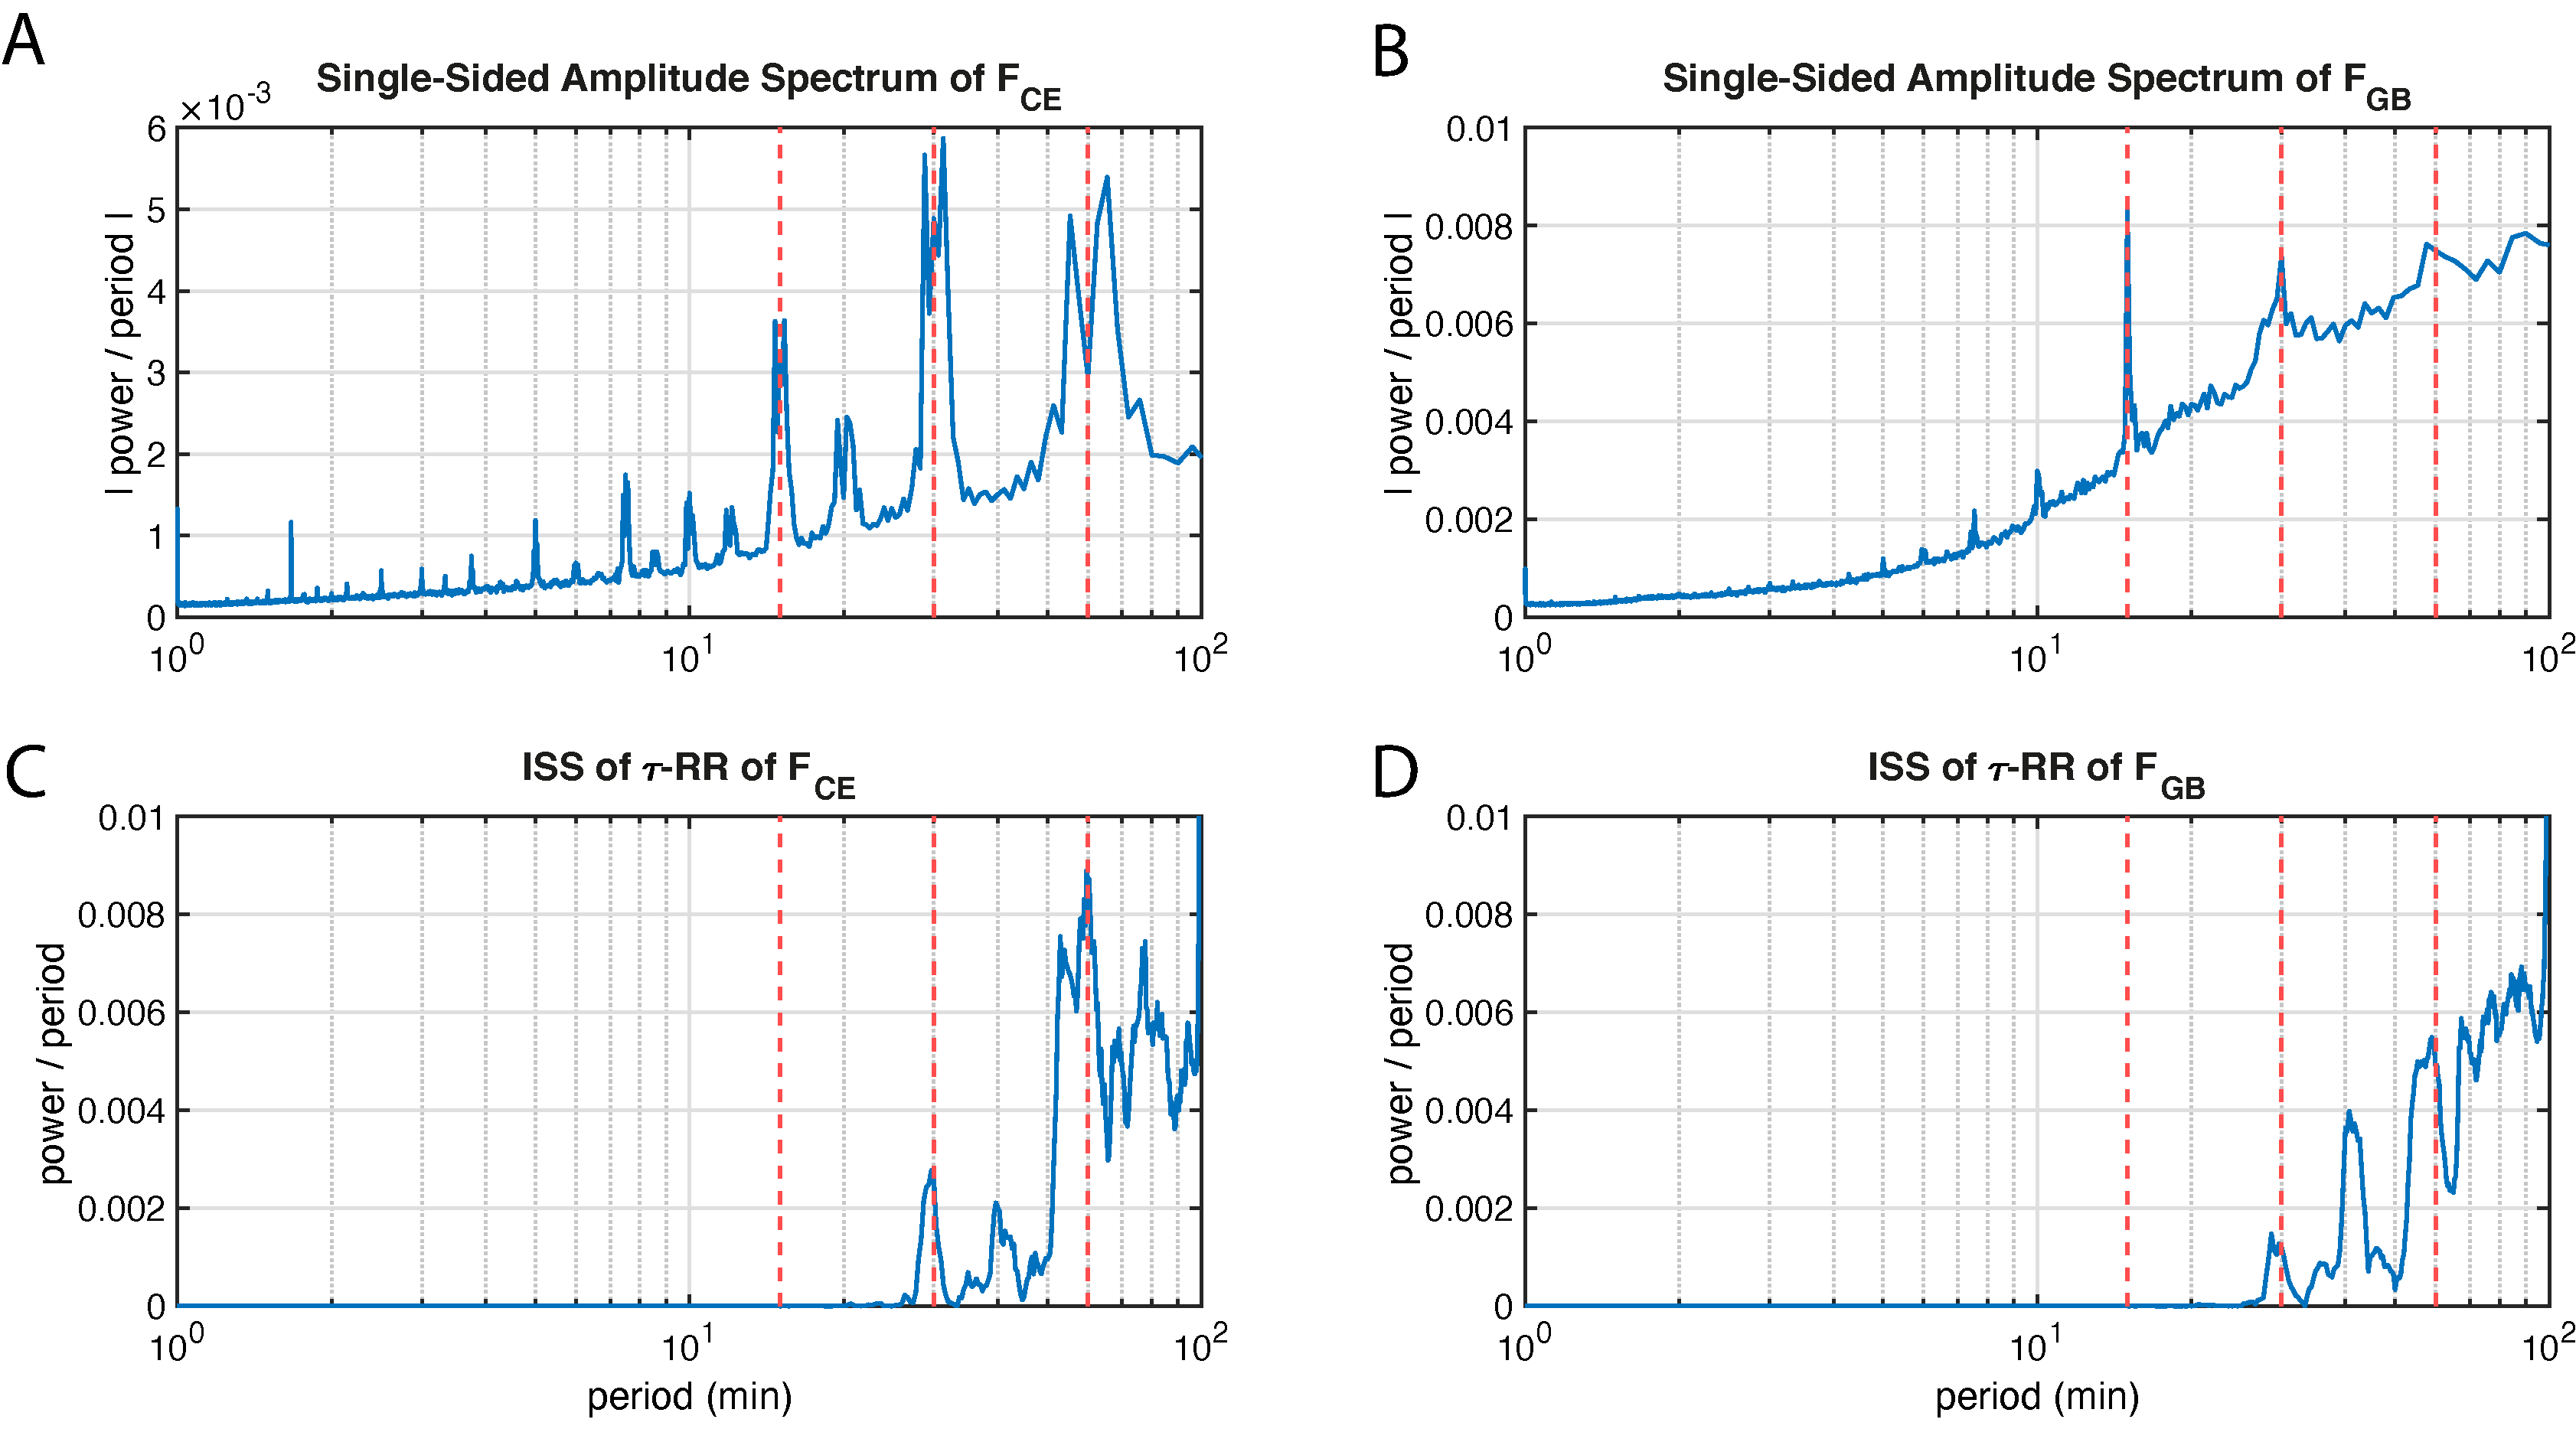
\includegraphics[width=\textwidth]{./figures/fig_power_grid_spectra}
 \caption{Averaged Fourier power spectra of recorded power grid frequency time series of \textbf{A} Central Europe (CE) and \textbf{B} Great Britain (GB) (see Appendix~\ref{sec_power_grid_appendix}). 
 The corresponding averaged inter-spike spectra of the according $\tau$-RRs, Eq.~\eqref{eq_tau_rr}, are shown in \textbf{C} and \textbf{D}, respectively. Vertical red dashed lines correspond to 
 $15$, $30$ and $60$ \si{min}. For technical details on the calculation of the spectra shown, the reader is referred to the Appendix~\ref{sec_power_grid_appendix}.}  
\label{fig_power_grid_spectra}
\end{figure}

The Fourier frequency spectra for the Central Europe data in Figure~\ref{fig_power_grid_spectra}A, however, does not display sharp peaks exactly at $15$, $30$ and $60$ \si{min}, which may partly 
be explained by the leakage effect (for technical details on the calculation of 
the spectra shown, the reader is referred to the Appendix~\ref{sec_power_grid_appendix}). Especially the $30$ and $60$ \si{min} 
peaks are split into two adjacent peaks and the local minimum in between these ``double''-peaks correspond to the exact times. The Great Britain counterpart in Fig.~\ref{fig_power_grid_spectra}B 
has sharp peaks at $15$ and $30$ \si{min} and also ``local predecessor peaks'' for $30$ and $60$ \si{min} at the same positions as in panel A. 
In contrast, the $15$ \si{min} peak is completely absent from the inter-spike spectra of the $\tau$-RRs of the frequency data (Fig.~\ref{fig_power_grid_spectra}C,D), but these show sharp peaks 
at $30$ and $60$ \si{min} (there is no leakage effect due to the proposed decomposition technique). 
In front of these peaks, smaller local peaks can be seen, which correspond to the local peaks of the Fourier power spectra at $28$ and $55$ \si{min}, respectively.
Moreover, there is an additional peak at 
$40$ \si{min} for both datasets, which is absent in the Fourier spectrum and which is not a multiple of the missing $15$ \si{min} peak. The position and magnitude of the peaks in the shown 
inter-spike spectra are robust to the chosen recurrence threshold, the regression method and its regularization as well as the sampling time of the original signal.

\todo[inline]{ISS appears first time here and is not explained. before it was written out.}
We interpret the results presented as follows. It should be noted firstly that ISS is not only capable to recognize the well-known periodicity in the power grid frequency because of the dispatching time, but also the ISS demonstrate more sharp peaks at this periodicity. The missing $15$ \si{min} in the inter-spike spectra is due to the much stronger autocorrelation at $30$ and $60$ \si{min} 
(see Fig.~\ref{fig_power_grid_time_series}B,D) and because these periods are integer multiples of $15$ \si{min} the inter-spike spectra are not able to detect it and the 
sparse regression ``drags'' the $15$ \si{min} periods into the mentioned $30$ and $60$ \si{min} peaks. Moreover, the inter-spike spectra, unlike the Fourier spectra demonstrates sharp peaks exactly 
at $30$ and $60$ \si{min}, i.e. during dispatches (not valid in case of the GB dataset). Eventually, here we have found a clear sharp peak at $40$ \si{min} which can occur 
because of any regular controls in a power grid, and can be a hint to develop the existing stochastic processes to model precisely the power grid frequency \cite{gorjao2020data}. 



%%%%%%%%%%%%%%%%%%%%%%%%%%%%%%%%%%%%%%%%%%
\subsection{Evolutionary inter-spike spectra of Earth's orbit data}

When applying the proposed inter-spike spectrum to the $\tau$-RR of a time series we expect additional frequency/period information, due to the fact that the recurrence plot (RP), 
Eq.~\eqref{eq_rp_definition}, and its corresponding $\tau$-RR, Eq.~\eqref{eq_tau_rr}, visualize the trajectory of the embedded time series in an embedding space of higher dimension. 
However, given a sufficient embedding of the time series, we would also expect that major frequencies/periods of the non-embedded time series are incorporated in the RP, its $\tau$-RR, 
and eventually in the inter-spike spectrum of the $\tau$-RR. In order to demonstrate this we apply the inter-spike spectrum to the freely available eccentricity time series of \citet{Laskar2011}. 
This astronomical computation of the orbital motion of the Earth (here we focus on the eccentricity only) has a clear expectation value of the incorporated frequencies/periods. The three leading 
eccentricity cycles of 405 kyr period, 95 kyr period and 124 kyr period are well known in palaeoclimate studies \cite{Laskar2004,Westerhold2020}. Our aim in this section is to show that the inter-spike spectrum 
of the $\tau$-RR of the embedded eccentricity time series will reflect these cycles in a similar fashion as the Fourier power spectral density of the non-embedded eccentricity time series. We will further 
show that Fourier-transforming the $\tau$-RR instead of applying the proposed inter-spike spectrum will lead to non-satisfying results, since the spiky $\tau$-RR excites a variety of harmonics in 
the corresponding Fourier spectrum (cf. Section \ref{sec_tau_rr_intro}). We use a time series which covers the past \mytilde $67$ Mio.~years (Myr), with a total length of $N=13,421$ samples and a 
sampling period of $\Delta t= 5,000$.

First we compute an evolutionary short time FT using a windowsize of $ws=1,000$ samplepoints ($\equiv 5$ Myr) shifted by unity and a 
Hamming window. The spectrogram reveals the expected periods mentioned, which are highlighted and clearly visible (Fig.~\ref{fig_laskar_spectra}A). 

\begin{figure}
 \centering
 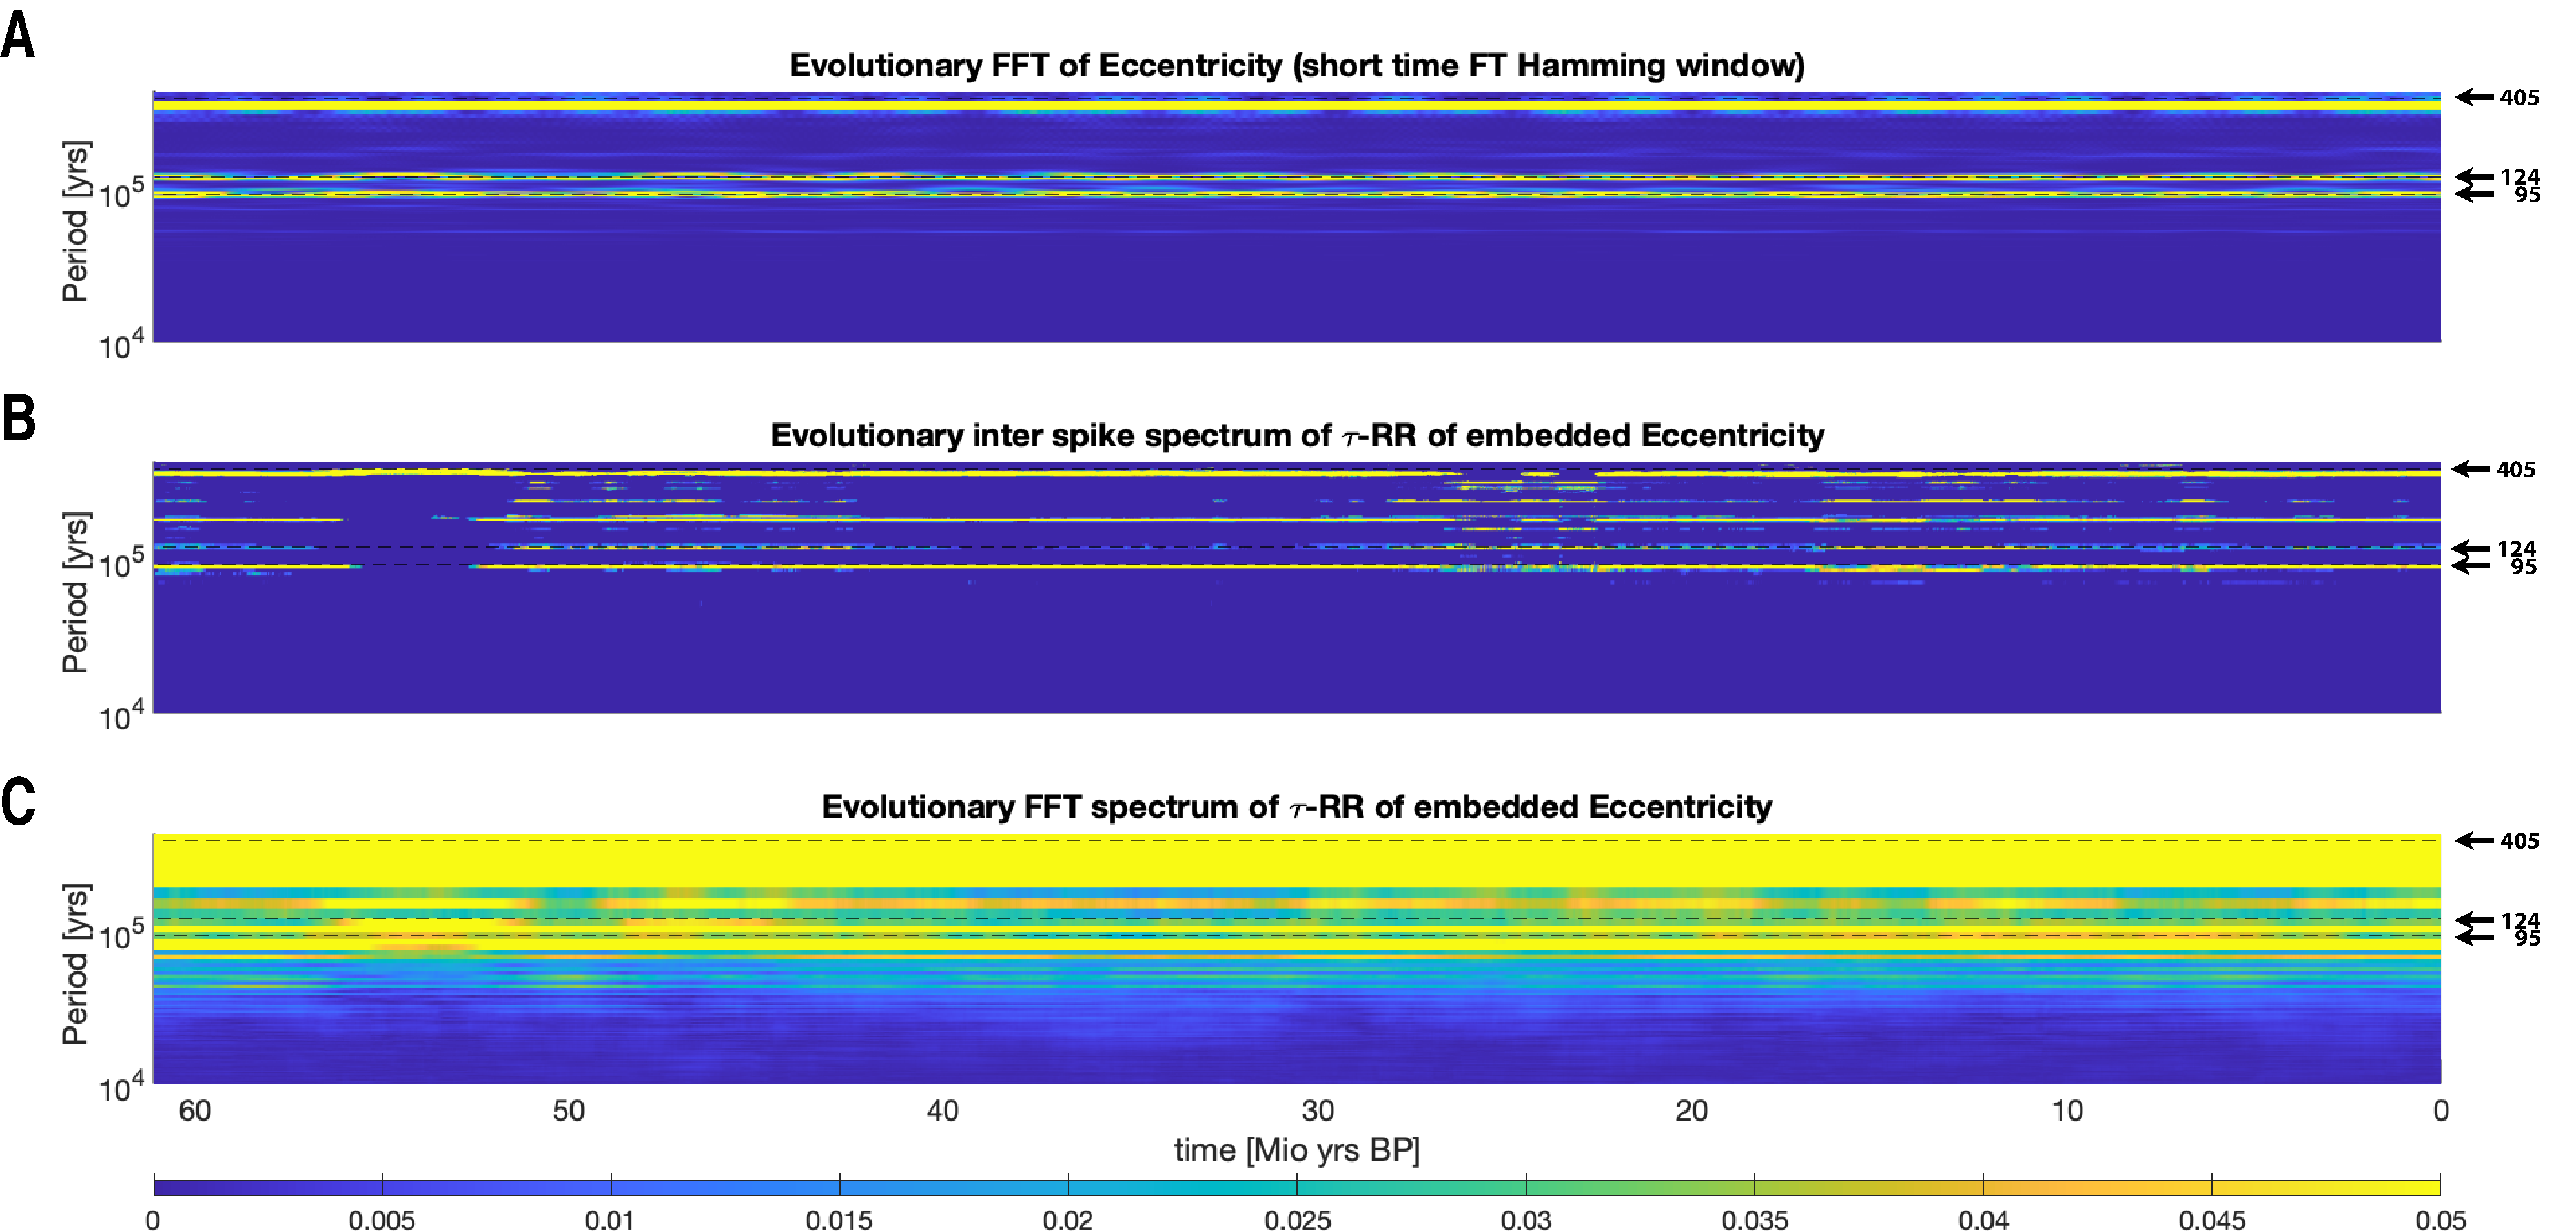
\includegraphics[width=\textwidth]{figures/fig_laskar_spectra}
 \caption{\textbf{A} Evolutionary Fourier power spectra of eccentricity time series. \textbf{B} Inter-spike spectrogram of the $\tau$-recurrence rate of the eccentricity time 
 series and \textbf{C} its Fourier spectrogram. Horizontal black dashed lines highlight the analytically expected orbital periods of $405$, $124$ and $95$ kyrs. 
 For comparability, in all cases the spectra aligned in the columns of the shown plots are normalized to probabilities (sum of unity for 
 each power spectrum). For further computational details, please refer to the main text.}  
\label{fig_laskar_spectra}
\end{figure}

\noindent Then we construct the inter-spike spectrogram of the $\tau$-RR by first determining an appropriate embedding. By using a recent Tree-Embedding-Ansatz \cite{Kraemer2022} we minimize the 
\textit{false nearest neighbor} statistic \cite{hegger1999} and use the continuity statistic \cite{pecora2007} for potential delays. Eventually we obtain an $8$-dimensional embedding 
with delays $\tau s=[0, 18, 36, 48, 62, 101, 114]$ (in sampling units) for the entire time series. Similar to the preceding approach we embed the time series with these embedding parameters 
on windows of size $ws=1,200$ and a unity shift.\footnote{We use a slightly larger window here than in the short FT, because the embedding causes a ``loss'' of data points and we want to 
cover similar time spans.} The RPs are computed on these embedded trajectories with a fixed recurrence threshold corresponding to $10\%$ global recurrence rate \cite{kraemer2018} 
and the inter-spike spectra of the corresponding $\tau$-RRs is obtained by using STLS regression (see Section \ref{sec_tau_rr_method}) and a regularization threshold corresponding to 
$\rho=0.9$ accordance of $\tau$-RRs and re-composed signals. We only use the first $200$ data points of the $\tau$-RR (covering a time span of $1$ Myr). 
The spectrogram also highlights the $95$, $124$ and $405$ kyr periods as expected (Fig.~\ref{fig_laskar_spectra}B). 
Additional power is distributed in its harmonics at $190$ and $248$ kyr periods. Finally, the standard FT with a Hamming window of the same $\tau$-RRs used to obtain the inter-spike 
spectrogram in panel B, yields a smeared spectrogram which does not reflect the expected periods, but rather suffers from the spike train behavior, i.e., many excited harmonics, of the 
FT described in Section \ref{sec_tau_rr_intro} and Fig.~\ref{fig_tau_rr_dirac_comb}. The shown results are robust to a change of embedding parameters and windowsizes. However, a too low 
regularization threshold smears the clear spectrogram in panel B.


%%%%%%%%%%%%%%%%%%%%%%%%%%%%%%%%%%%%%%%%%%
\section{Discussion}\label{sec_tau_rr_discussion}

We have successfully used the idea of transforming the $\tau$-RR for the detection of bifurcations in the Logistic map. By constructing appropriate surrogates of the inter-spike spectra, 
and, thus, a null model, the number of significant peaks in the inter-spike spectrum correlated well with the positive Lyapunov exponent. This measure was also able to resolve 
period-doubling bifurcations. However, we have to admit this way the detection of a bifurcation is only possible when the additional period(s) is not an integer multiple of the former period(s). 
This behavior is described in the application to the R\"ossler system, where we explicitly showed the different inter-spike spectra for period-2, period-3, and chaotic dynamics.
Further development might potentially incorporate the mutual distance of peaks in the spectrum for a better correlation to the Lyapunov exponent. The inter-spike spectra of power grid 
frequency data illustrate that our proposed method may serve as a valuable source of information in addition to a standard Fourier analysis. And last but not least, we showed that our approach 
really incorporates frequencies, which are apparent in the Fourier spectrum of the signal, by applying it to analytically derived eccentricity data, where the dominant frequencies are well 
known.

We discuss some more technical details in the following, which will also affect any application of the proposed method. 
First of all, the number of required basis functions 
$M = \sum_{i=1}^{\ceil*{N/2}+1}i$ for an input signal of length $N$ is the crucial bottleneck of this approach, which is why it does not show good scaling behavior. The subsequent sparse 
regression, therefore, gets computationally intensive for $N>1,000$. Depending on the memory of the computer used, input signals $N>2,000$ usually do not work anymore. This means that signals 
often need to get downsampled as a preprocessing step (e.g., see Appendix \ref{sec_power_grid_appendix}). Second, the regularization parameter $\alpha$ for the regression is a crucial free parameter. 
As described in Sect.~\ref{sec_tau_rr_method}, our idea in this paper is to select the $\alpha$ such that the re-composed signal $\tilde{\vec{s}}=\bfX^T\hat{\boldsymbol\beta}$ matches a 
given (Pearson) correlation coefficient $\rho_{\vec{s},\tilde{\vec{s}}}$ between the original signal $\vec{s}$ and itself. This ensures that $\alpha$ adjusts itself to the data as well as to the 
used regression method. We found that this increases the comparability of different spectra, especially when performing a running window approach in order to obtain an evolutionary spectrogram 
(Fig.~\ref{fig_laskar_spectra}). 
However, the two different sparse regression algorithms we encountered in this article (LASSO and STLS) yield different results for the same desired $\rho_{\vec{s},\tilde{\vec{s}}}$. 
Even if the spectra obtained in this way look qualitatively similar, they are not always quantitatively similar. The reason for this 
is that $\rho_{\vec{s},\tilde{\vec{s}}}$ is not a smooth function of $\alpha$ in case of STLS, due to the hard-thresholding involved \cite{Brunton2016}, which is shown in Fig.~\ref{fig_regularization}.
Third, when adopting our idea of applying the inter-spike spectrum to the $\tau$-recurrence rate of the signals state space trajectory, the embedding process induces additional free parameters.  
This is not a drawback of the proposed decomposition method, but rather a drawback of applying this technique to the $\tau$-recurrence rate of the system, which was the main motivation for 
developing the proposed method. As a very last remark, we draw attention to the fact that sparse regression can be transformed into sparse logistic regression when the signal we would like to transform is binary.


%%%%%%%%%%%%%%%%%%%%%%%%%%%%%%%%%%%%%%%%%%
\section{Conclusion}\label{sec_tau_rr_conclusion}

A novel decomposition technique is proposed that yields the \textit{inter-spike spectrum}. The method decomposes any arbitrary signal into basis functions which consist of (lagged) Dirac 
combs (DC) of different inter-spike period. The loading for each period is obtained by a regularized regression, which promotes sparsity in its solution. We chose LASSO or a sequentially 
thresholded least squares regression STLS in this letter. Since there are 
$M = \sum_{i=1}^{\ceil*{N/2}+1}i$ basis functions for a signal of length $N$ the regression can get computationally intensive for $N>1,000$. When plotting the computed loadings as a function 
of the period (or frequency) the inter-spike spectrum is obtained. A disadvantage is that the transformation is not invertible. An advantage is that there is no leakage effect.
Although this novel spectrum is superior to an ordinary FFT-based power spectrum when the signal has a spike-train-like appearance, the authors suggest that this method should 
be considered 
as an additional source of information but not as a substitute for ordinary Fourier analysis. 
Due to the sparse regression underlying the method, there is no unique inverse of the transformation and the regularization parameter plays a crucial role and determines the 
appearance of the obtained inter-spike spectrum. Moreover, similar to the Nyquist frequency barrier in the Fourier Transform which sets a lower bound for the corresponding wave period, here 
the maximum considered inter-spike period is bounded by $T_{\text{is}}^{\text{max}} = \ceil*{N/2}+1$.

The invention of the proposed method has been motivated by the idea of transforming $\tau$-recurrence rate signals ($\tau$-RRs) into their frequency domain. 
This general idea \cite{Zbilut2008} allows for a frequency analysis of high dimensional systems, because the RP is a representation of the system's state space trajectory.   
The $\tau$-RR of a recurrence plot (RP) usually has a spiky shape, especially for map-like data, and the inter-spike spectrum can reliably reveal the system's dominant frequencies, 
which is not possible when Fourier transforming the $\tau$-RR or the underlying signal itself. Since the position of the peaks 
in the $\tau$-RR are not sensitive to noise, the corresponding inter-spike spectrum also yields robust results in the presence of noise. 

We could think of a broad range of applications of the proposed idea. The inter-spike spectrum itself can serve as a valuable tool for the analysis of any sort of 
spike-train-like data. On the other hand, the inter-spike spectrum of the $\tau$-RR of a signal can serve as a generalized, nonlinear frequency analysis tool for complex systems. 
When there is only a subset of state variables available, the state space has to be reconstructed as a pre-processing step. Recent findings \cite{Kraemer2021,Kraemer2022} show that 
this reconstruction process can be reliably automated and applied to multivariate data as well. This would allow for a ``running window'' approach, in order to detect transitions. 
Due to the mentioned computational constraints of our proposed method, a window size $w\leq 1,000$ would possibly suffice for most data, especially when it is map-like, i.e., not 
highly sampled. 


%%%%%%%%%%%%%%%%%%%%%%%%%%%%%%%%%%%%%%%%%%
\vspace{6pt} 


%%%%%%%%%%%%%%%%%%%%%%%%%%%%%%%%%%%%%%%%%%
\authorcontributions{Conceptualization, KHK and FH; methodology, KHK, FH and NM; software, KHK and FH; validation, KHK, FH, MA and NM; formal analysis, KHK; data curation, KHK and MA; writing---original draft preparation, KHK; writing---review and editing, KHK, FH, MA and NM; visualization, KHK; supervision, NM; project administration, JK; All authors have read and agreed to the published version of the manuscript.}

\funding{This work has been financially supported by the German Research Foundation (DFG projects MA4759/8 and MA4759/9).}

\dataavailability{The study that we present here is available as a fully reproducible code base
**Repository will be published and cited here, when accepted** and the method
will be available in the Julia language **Package will be published and cited here, 
when accepted** and as a MATLAB\textsuperscript{\textregistered} toolbox 
**Toolbox will be published and cited here, when accepted**.} 

\acknowledgments{
All computations have been carried out in MATLAB\textsuperscript{\textregistered} and the Julia language 
and made use of the packages \textit{DynamicalSystems.jl} \cite{datseris2018}, \textit{DifferentialEquations.jl} \cite{rackauckas2017}, \textit{Distances.jl} and 
\textit{OptimalTransport.jl} \cite{Zhang2022}.
}

\conflictsofinterest{The authors declare that they have no conflict of interest.} 

\clearpage
%%%%%%%%%%%%%%%%%%%%%%%%%%%%%%%%%%%%%%%%%%
%% Optional
\appendixtitles{yes} % Leave argument "no" if all appendix headings stay EMPTY (then no dot is printed after "Appendix A"). If the appendix sections contain a heading then change the argument to "yes".
\appendixstart
\appendix

\section{Exemplary models}
 
\subsection{Lorenz system}\label{sec_models_lorenz63}

\noindent The classical Lorenz-63 system \cite{lorenz1963} is defined as

\begin{equation}
\begin{array}{rcl}
\dot{x}&=&\sigma(y-x) \\
\dot{y}&=&x(r-z)-y \\
\dot{z}&=&xy - \beta z.
\end{array}
\label{eq_model_Lorenz63}
\end{equation}

\noindent For producing Fig.~\ref{fig_tau_rr_spectrum_example} we set the initial condition to $u_0=[0.0, 10.0, 0.0]$, used a sampling time of $\Delta t=0.01$ and discarded the first 
2,000 points of the integration as transients. The parameters have been set to 
$\sigma=10, \beta=8/3, \rho=28$ and we used a time series consisting of 6,000 samples.

\subsection{R\"ossler system}\label{sec_models_roessler}

\noindent The R\"ossler system \cite{roessler1976} is defined as
\begin{align}
\begin{array}{rcl}
\dot{x}&=&-y-z \\
\dot{y}&=&x+ay \\
\dot{z}&=&b+ z(x-c) .
\end{array}
\label{eq_model_roessler}
\end{align}
For producing Figs.~\ref{fig_tau_rr_example_roessler_noise} and ~\ref{fig_tau_rr_example_roessler}, the initial condition for producing panels \textbf{A} \& \textbf{B} was set to $u_0=[0.7, -1, 0.4]$ with a sampling time 
of $dt=0.05$ and in case of panel \textbf{C}, $u_0=[-0.1242, -2.5415, 0.2772]$ with a sampling time of $dt=0.1$. The first $5,000$ samples were discarded as transients and trajectories of length $N=5,000$ were 
obtained from which we computed the RPs and the corresponding $\tau$-RRs. For the inter-spike spectra only the first $1,000$ values of the $\tau$-RRs were considered.

\section{Power grid frequency time series}\label{sec_power_grid_appendix}

The raw frequency time series have length $\tilde{N}_{\text{CE}}=58,752,000$ and $\tilde{N}_{\text{GB}}=31,622,400$ with sampling times $\Delta t_{\text{CE}}=0.2$\si{s} and 
$\Delta t_{\text{GB}}=1$\si{s}, respectively. GB frequency data was measured during 2016, and has been gotten from \cite{GB}. CE frequency data belongs to 2017 and has been gotten from \cite{haehne2018footprint}.
  
We downsampled these time series to a sampling time of $\Delta t_{\text{CE}}= \Delta t_{\text{GB}}=20$\si{s}, which led to total time series lengths of 
$N_{\text{CE}}=587,520$ and $N_{\text{GB}}=1,581,120$ which we used for the further analysis.

\begin{figure}
 \centering
 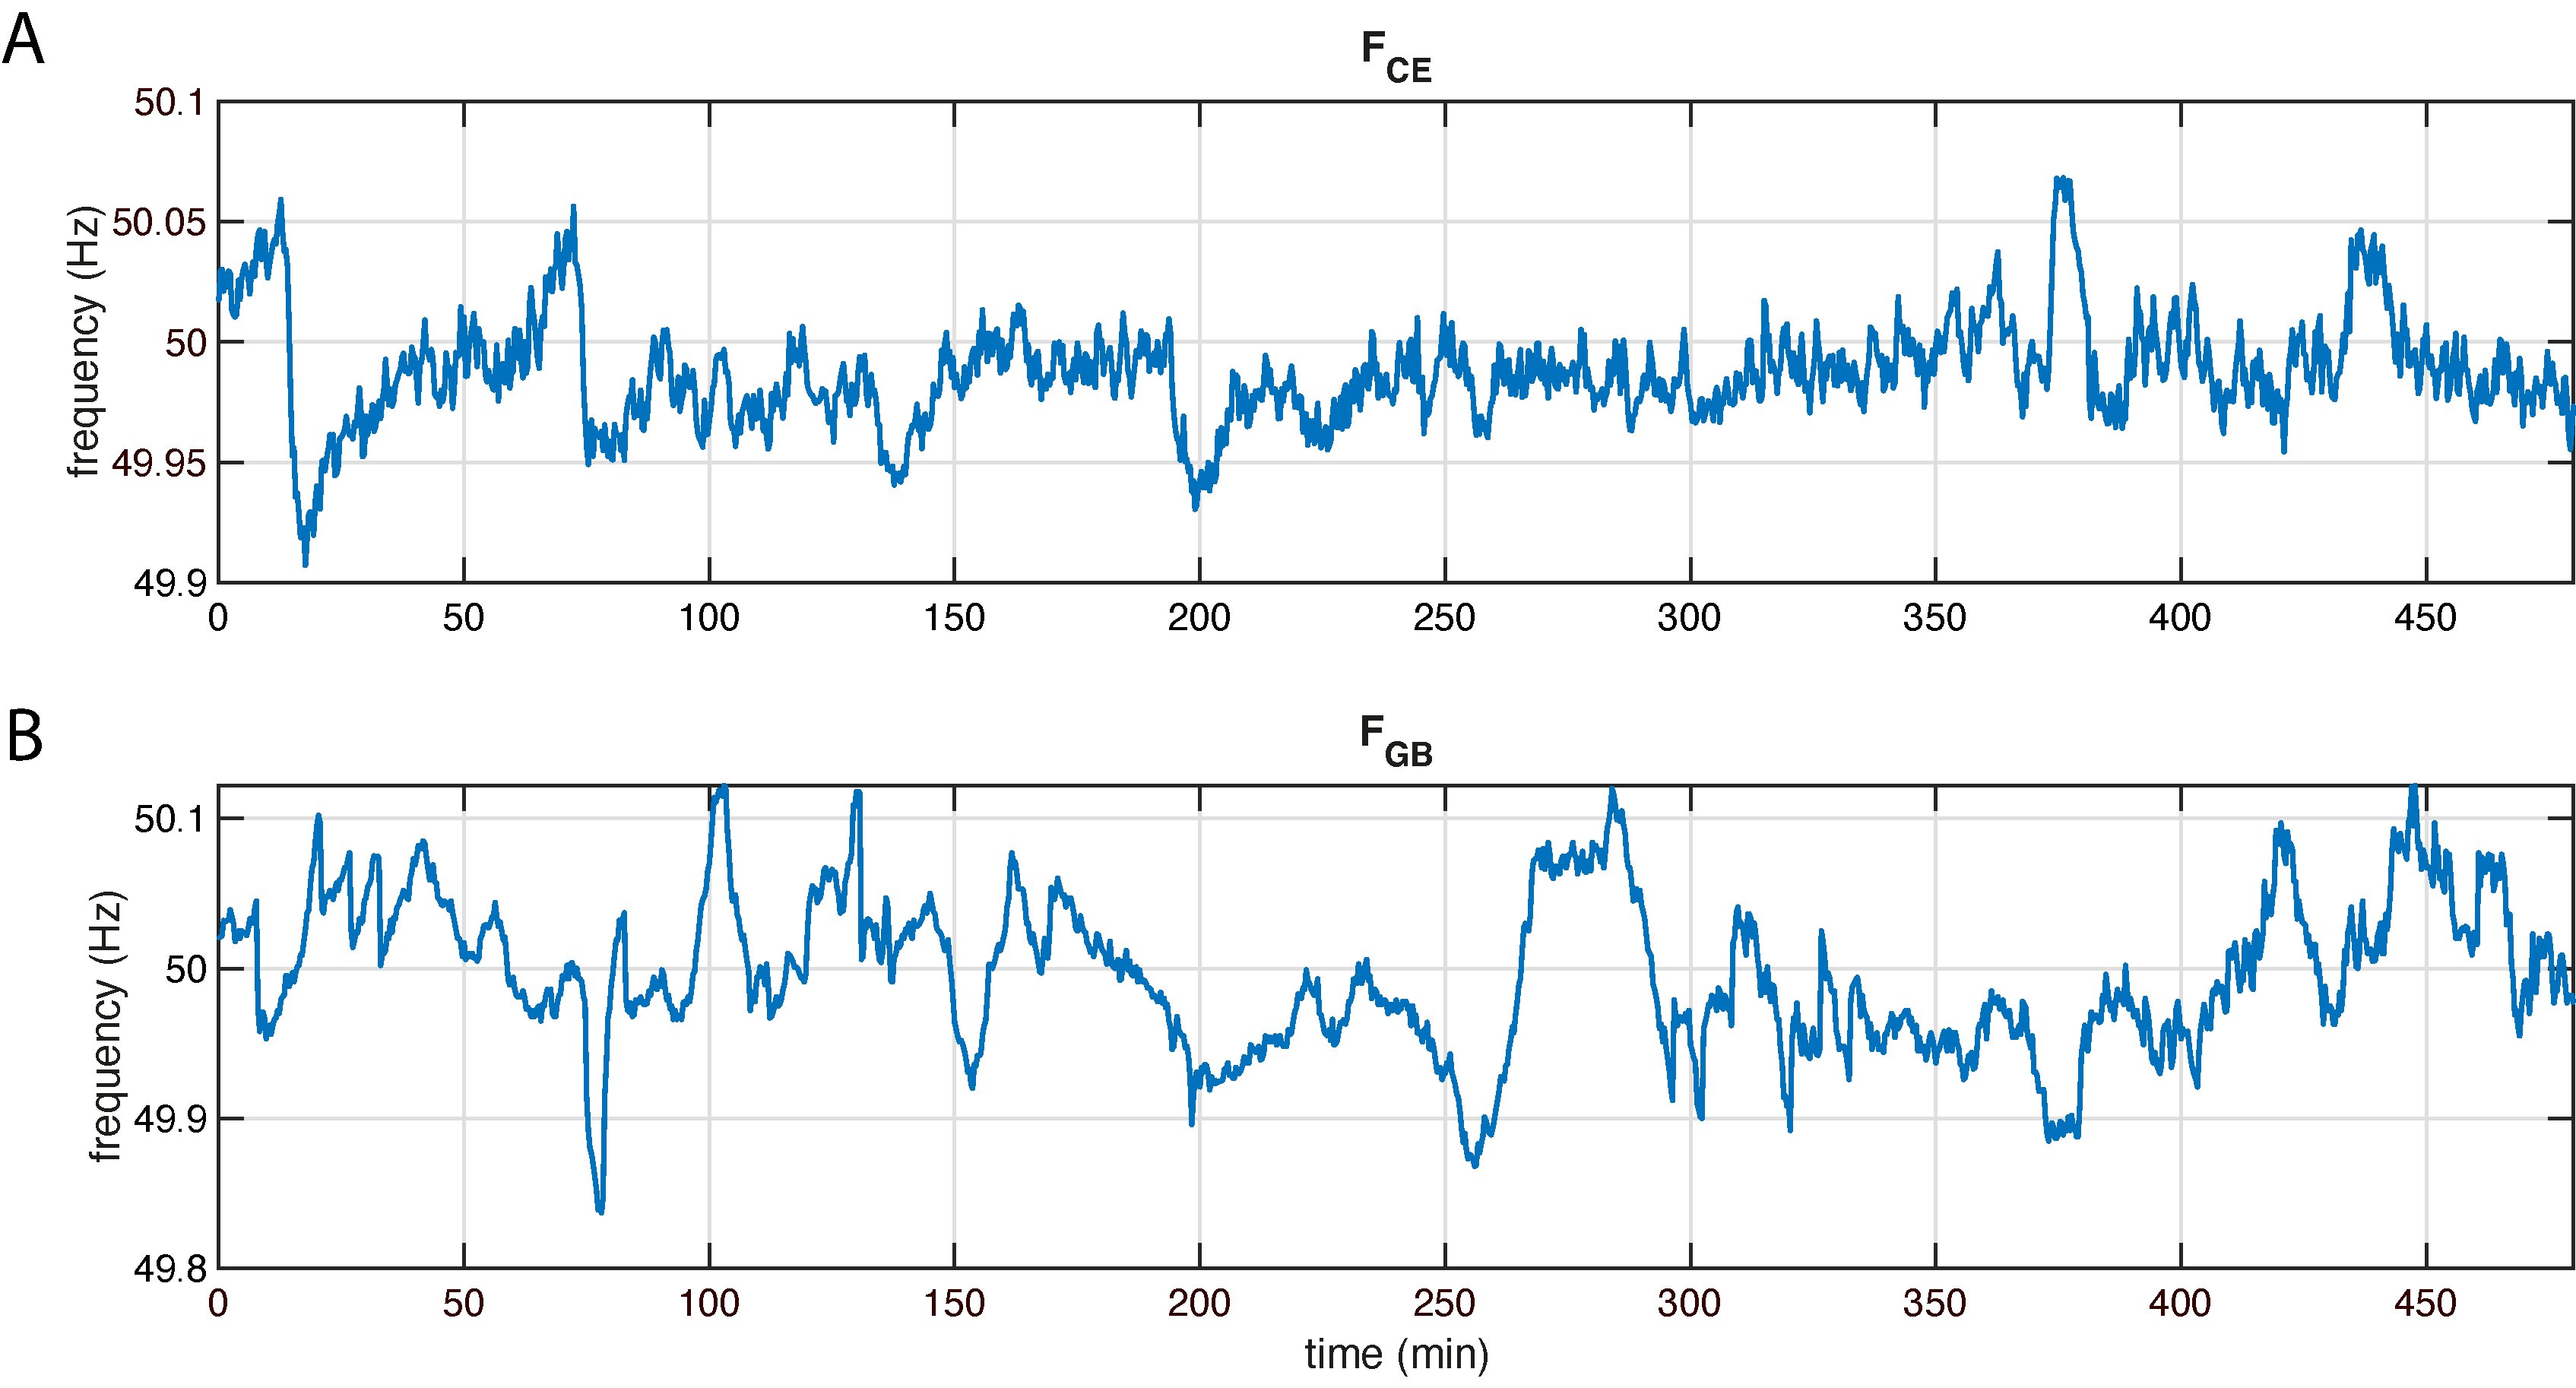
\includegraphics[width=\textwidth]{./figures/fig_power_grid_time_series}
 \caption{Subset of the frequency time series of \textbf{A} Central Europe (CE) \cite{haehne2018footprint} and \textbf{C} Great Britain (GB) \cite{GB} along with their autocorrelation functions in \textbf{B} and 
 \textbf{D}, respectively. The normalized autocorrelations in \textbf{B}, \textbf{D} have been computed on the entire time series, wheres as the subsets shown in \textbf{A}, \textbf{C} 
 contain only $1,441$ samples.}
\label{fig_power_grid_time_series}
\end{figure}

In this analysis we divided the time series into 
non-overlapping blocks of length $N_{\text{block}}=4,320$, covering a time span of $24$ hours. For each time series block we computed Fourier spectra and recurrence plots (RPs), 
Eq.~\eqref{eq_rp_definition}, along with their $\tau$-RRs, Eq.~\ref{eq_tau_rr}. The RPs were obtained from a uniform 5-dimensional time-delay embedding of each time series with 
the delay set to the first minimum of the mutual information \cite{fraser1986,hegger1999} and a fixed recurrence threshold corresponding to 8\% recurrence rate was used in order 
to ensure comparability \cite{kraemer2018}. The first $600$ data points of the $\tau$-RRs were used for finally obtaining inter-spike spectra with a LASSO regression and a 
regularization threshold corresponding to $\rho=0.95$ accordance of $\tau$-RRs and re-composed signals. The spectra shown in all panels of Figure~\ref{fig_power_grid_spectra} 
are averages over all blocks, following \citet{meyer2020identifying}.

\begin{figure}
 \centering
 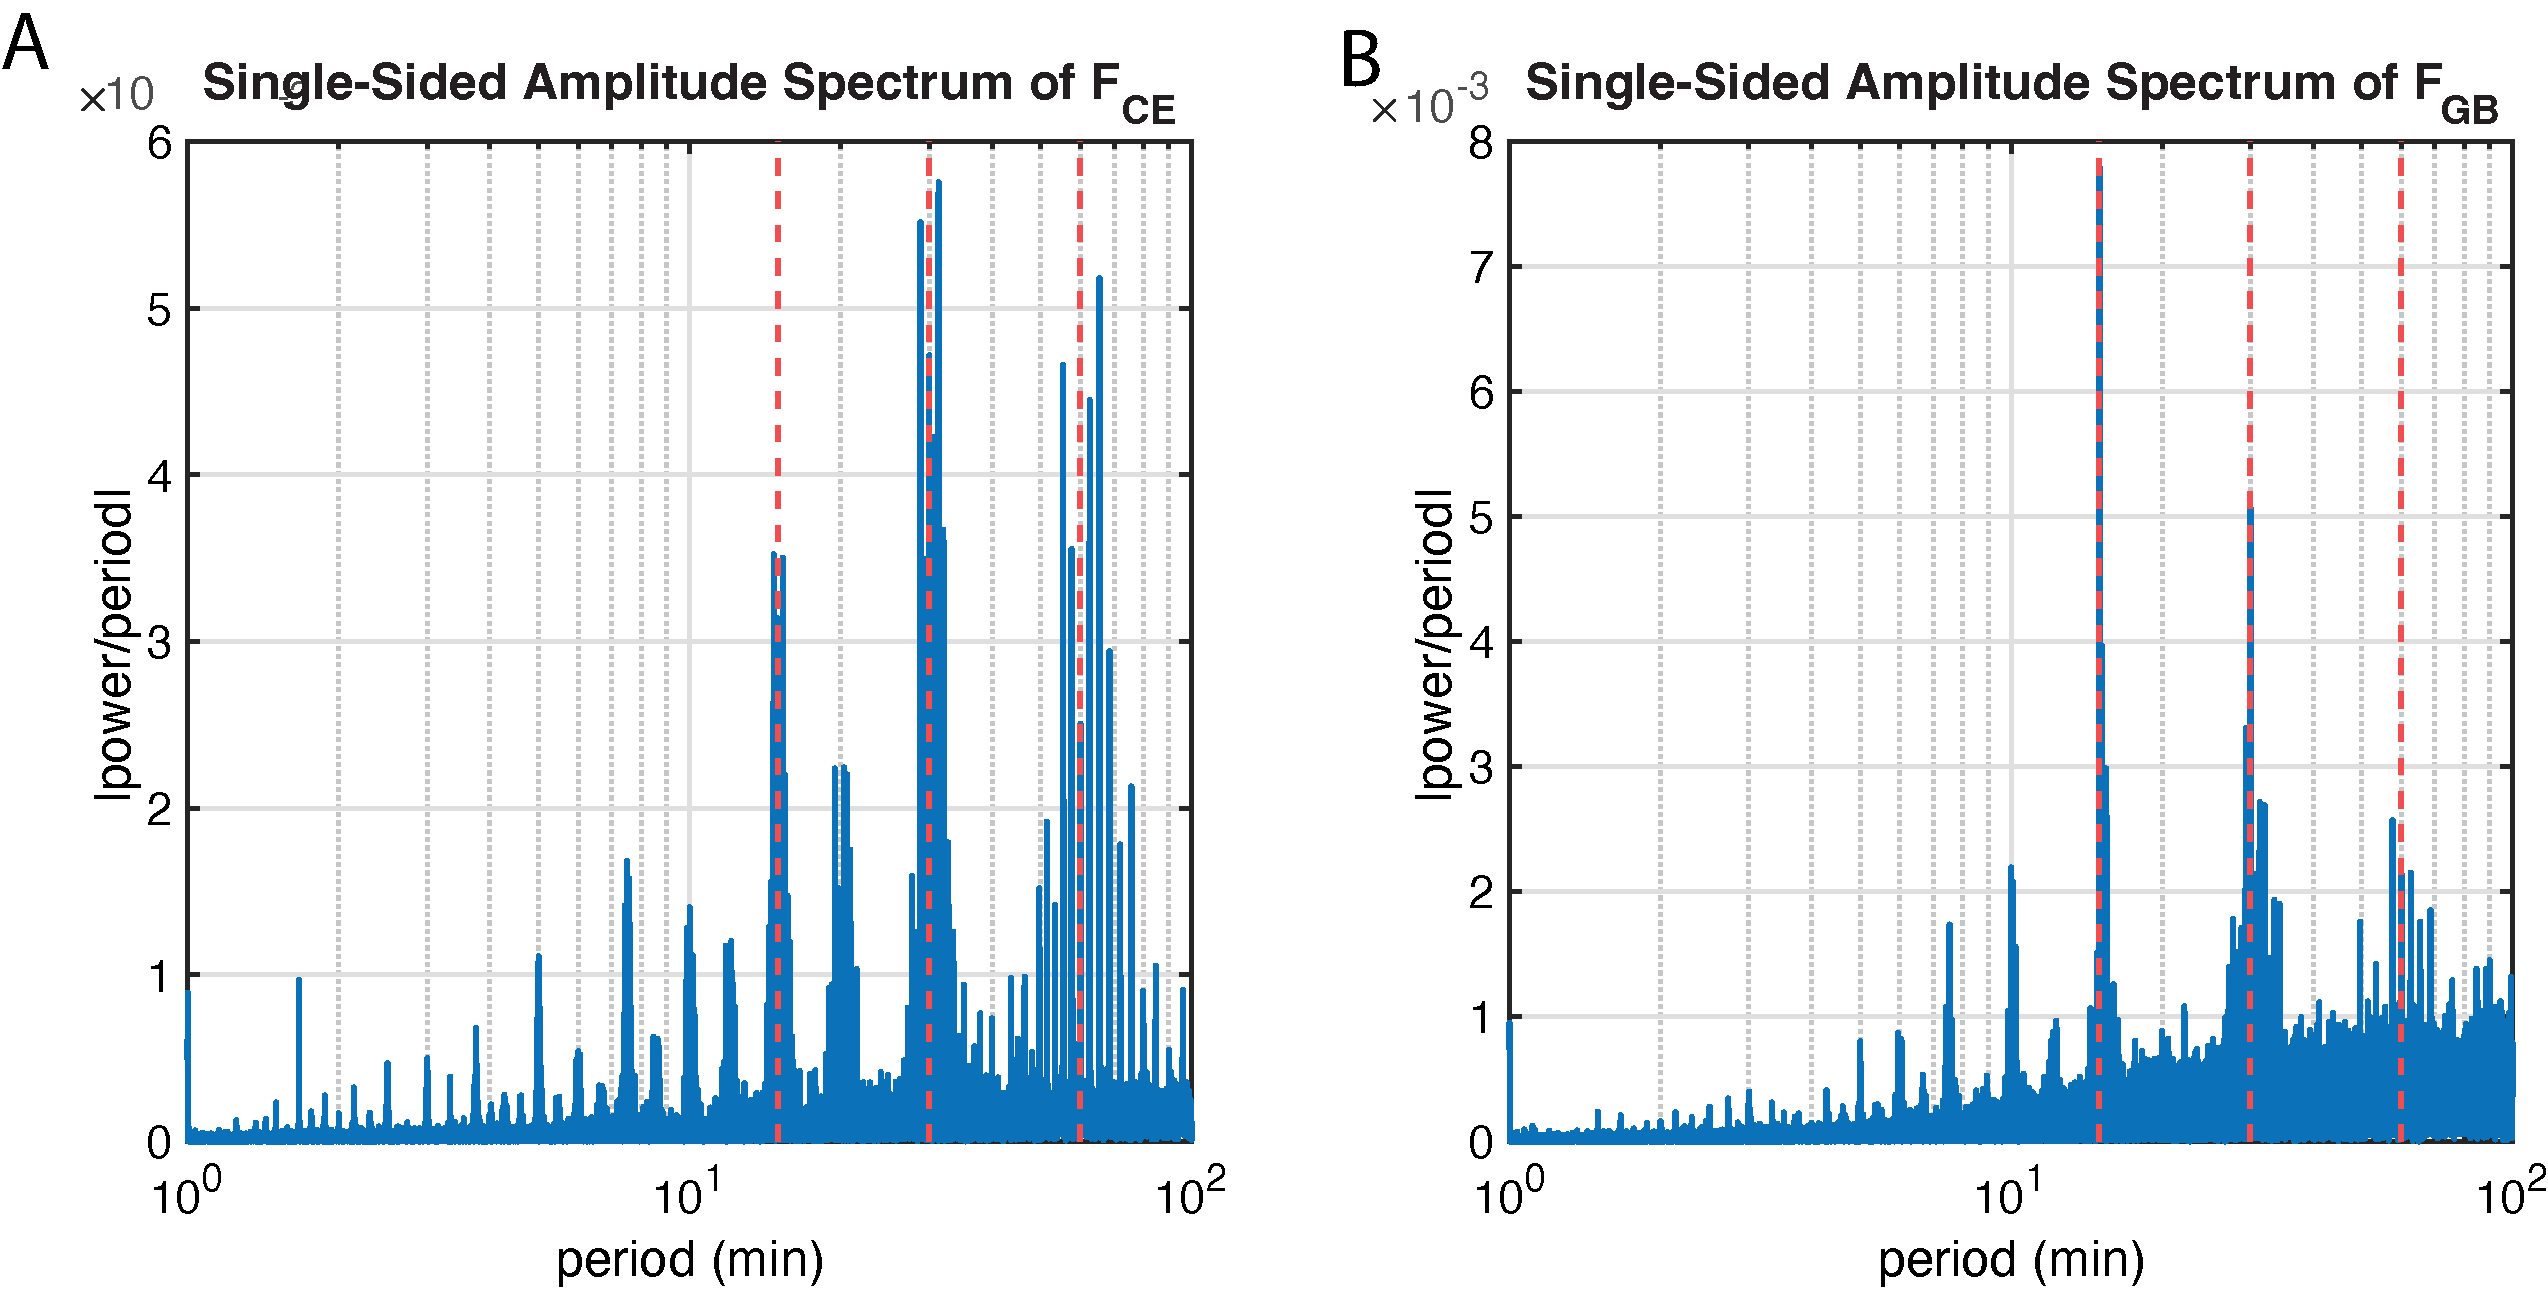
\includegraphics[width=\textwidth]{./figures/fig_power_grid_fft_full}
 \caption{Fourier spectra of the frequency entire time series from \textbf{A} Central Europe (CE), $N_{\text{CE}}=587,520$ and \textbf{B} Great Britain (GB), $N_{\text{GB}}=1,581,120$. A subset of the underlying time series is shown in Fig.~\ref{fig_power_grid_time_series}.}
\label{fig_power_grid_fft_full}
\end{figure}

\clearpage

\section{inter-spike spectra for noisy R\"ossler system}

\begin{figure}[h!]
 \centering
 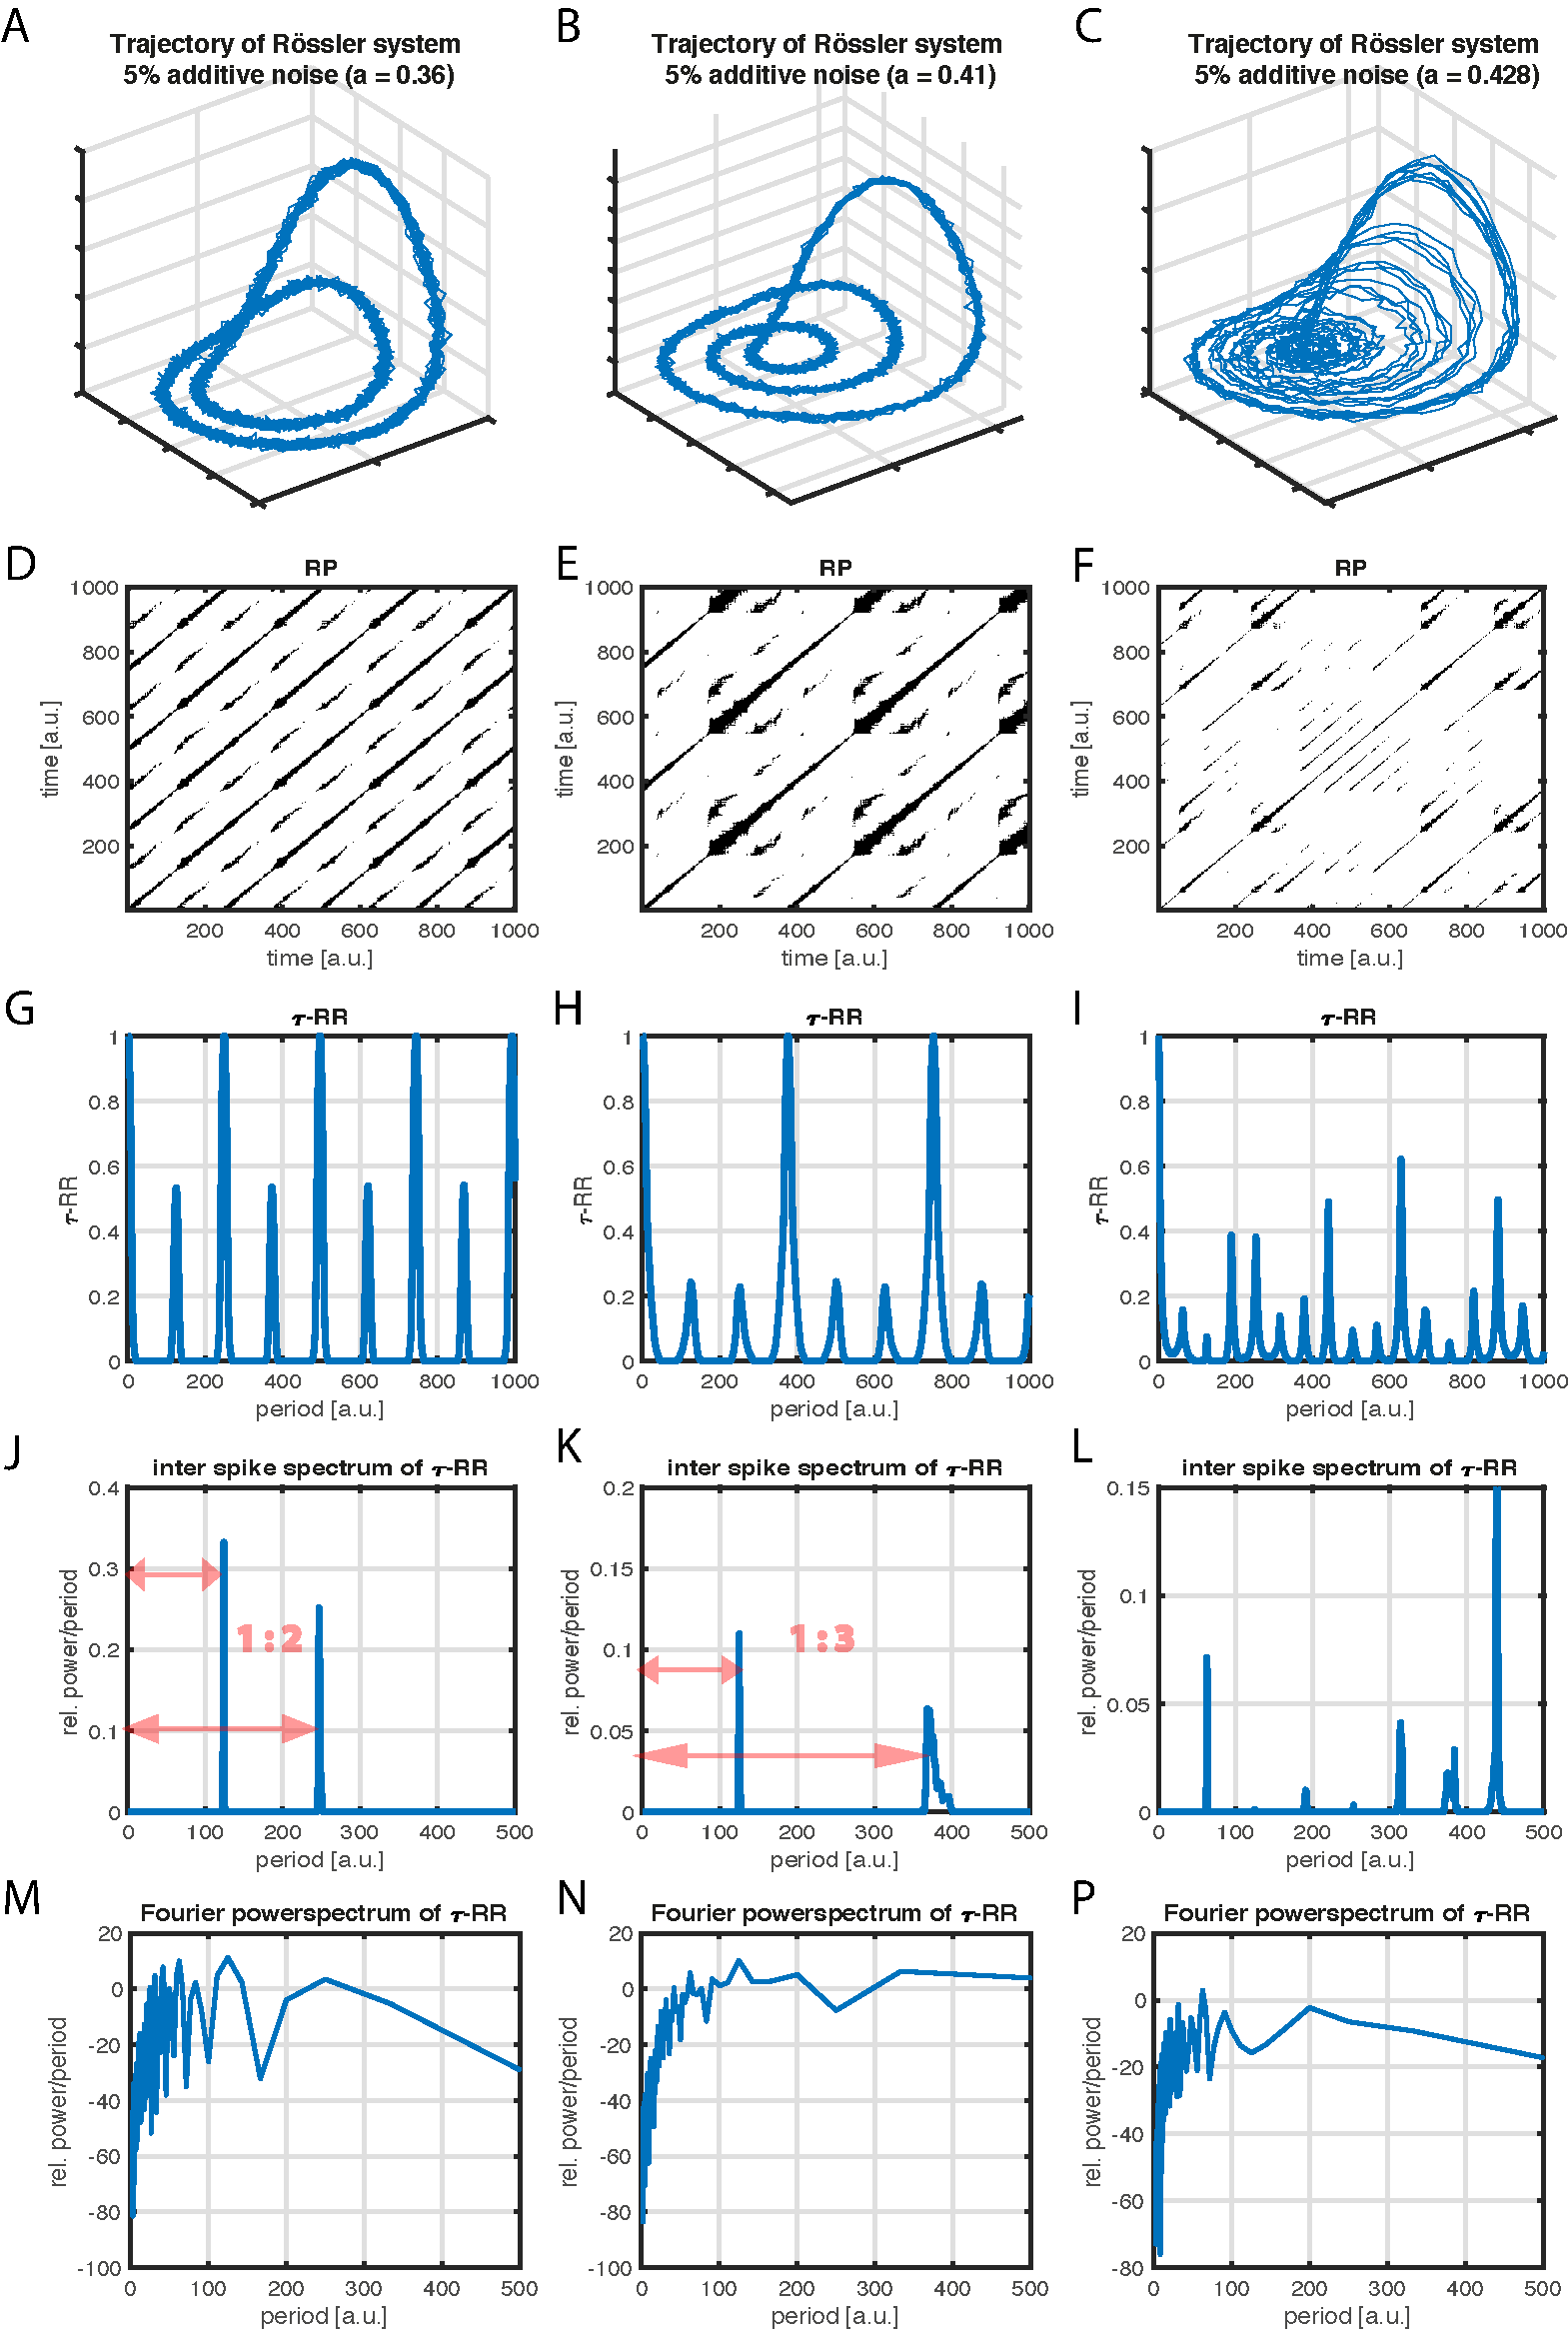
\includegraphics[width=0.9\textwidth]{./figures/fig_tau_rr_example_roessler_noise}
 \caption{Same as in Fig.~\ref{fig_tau_rr_example_roessler}, but here with 5\% additive Gaussian white noise on each component $x$, $y$ and $z$. The appearance of the inter-spike spectra 
 in \textbf{J, K, L}, and the Fourier spectra in \textbf{M, N, P} are unaffected by the additive noise.}
\label{fig_tau_rr_example_roessler_noise}
\end{figure}

\clearpage 

\begin{figure}[h!]
 \centering
 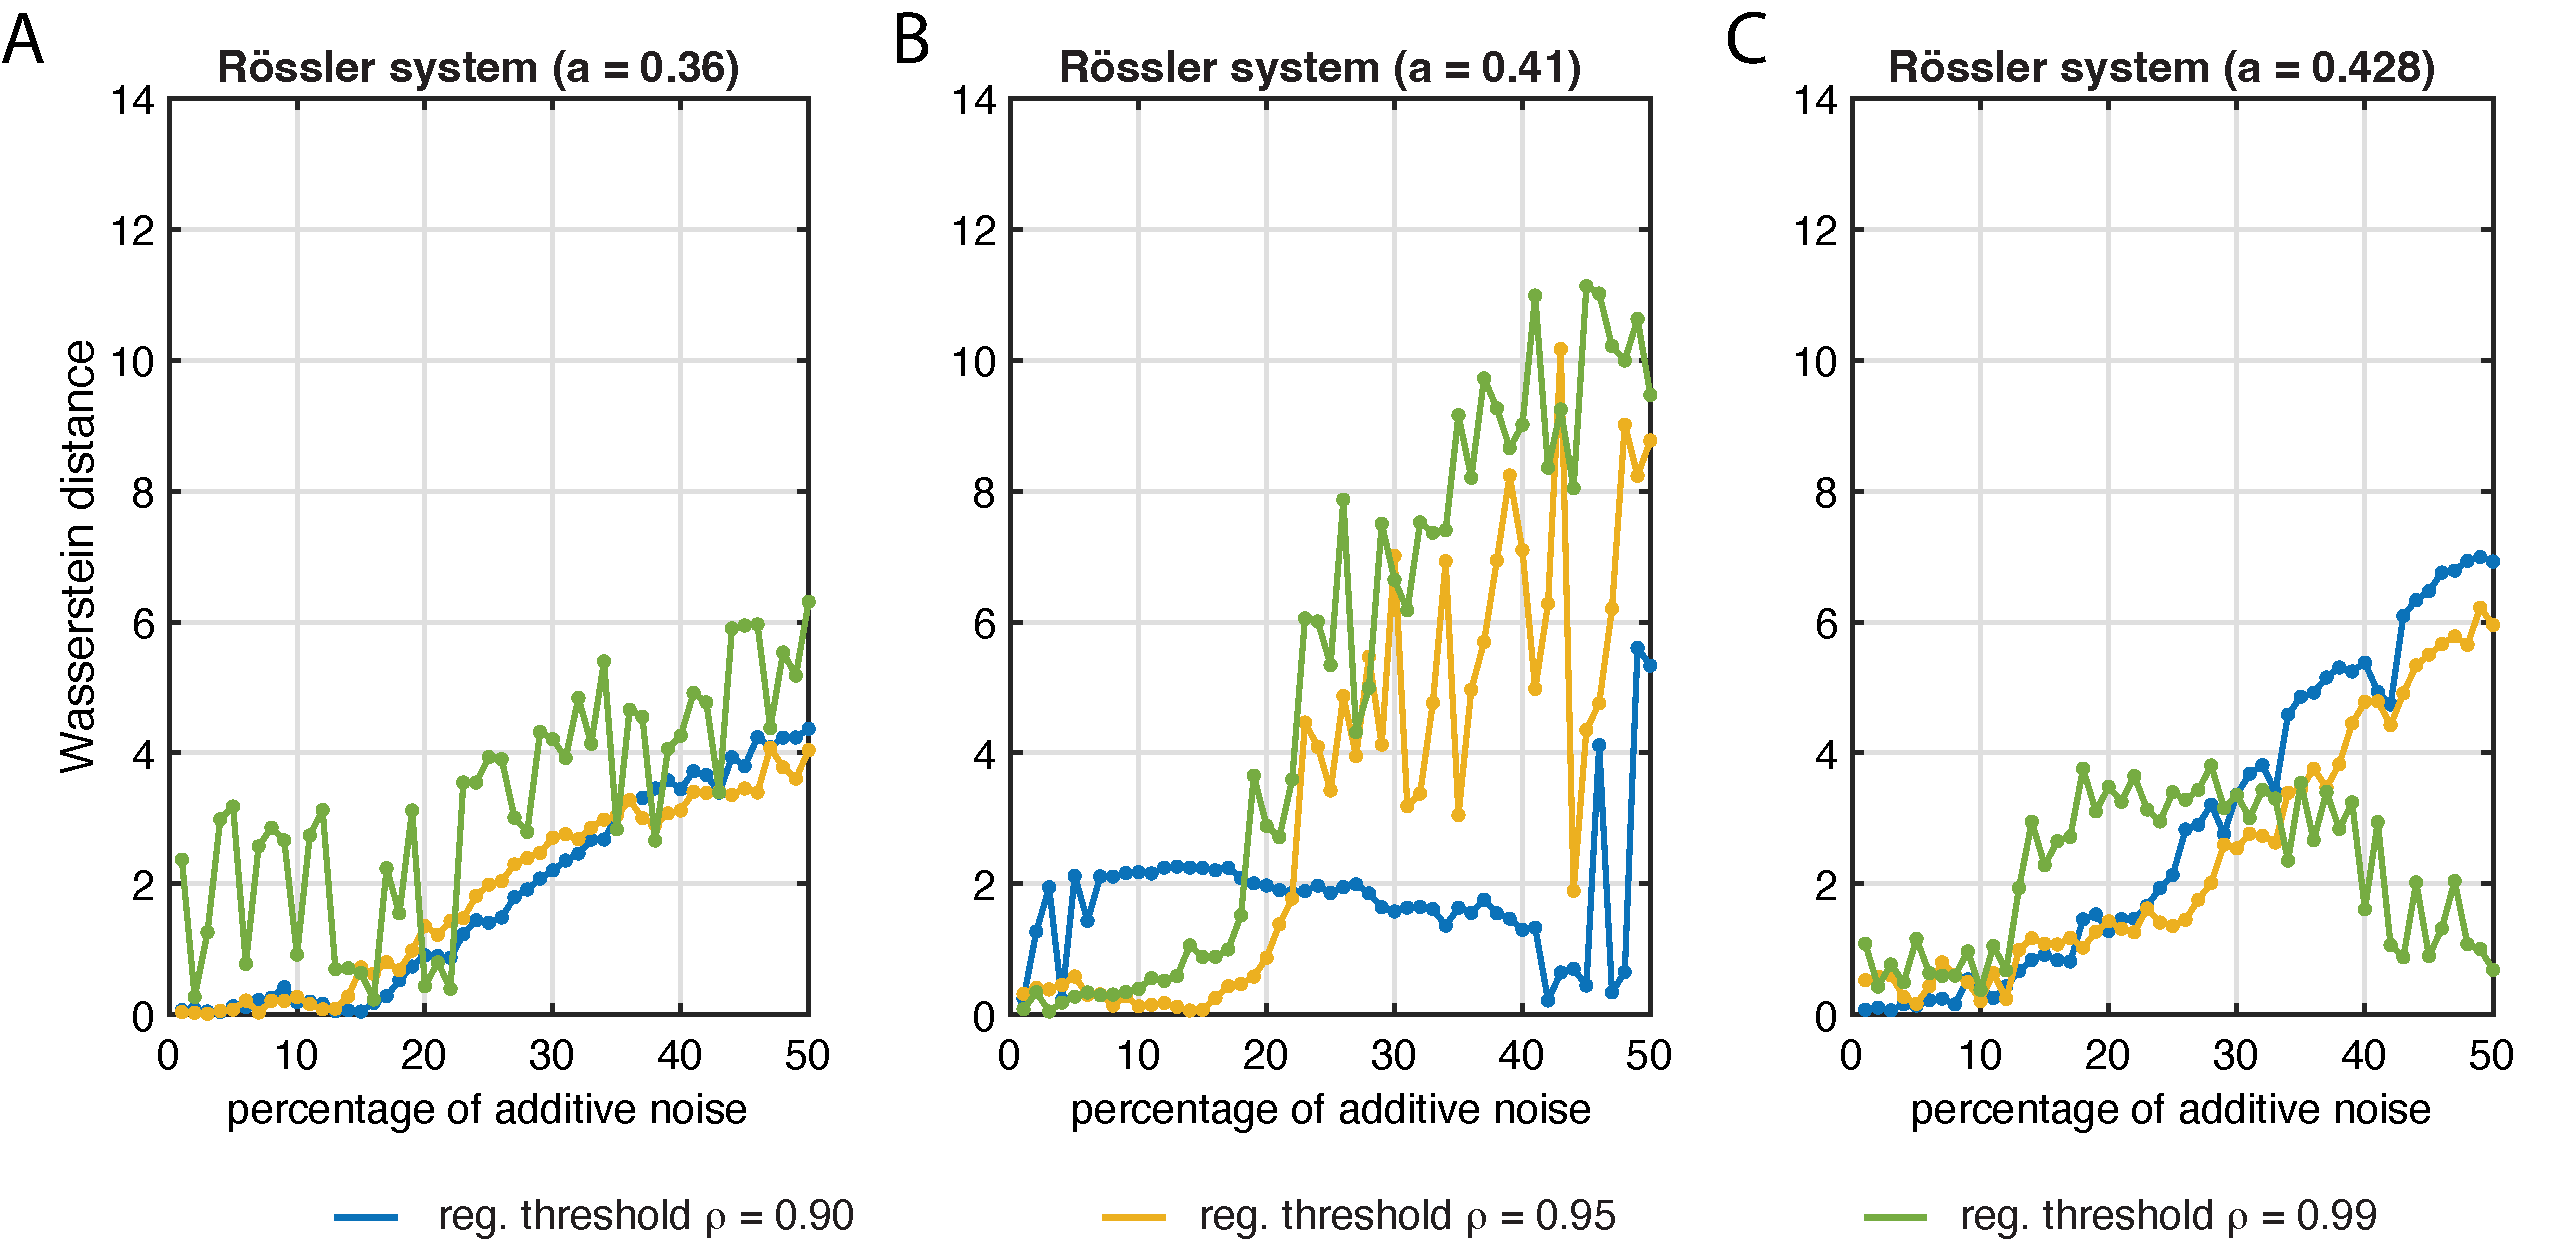
\includegraphics[width=0.9\textwidth]{./figures/fig_roessler_spectra_distances}
 \caption{Wasserstein distances for the obtained inter-spike spectra of the $\tau$-RRs for additive noise levels up to 50\% for the discussed R\"ossler dynamics, 
 \textbf{A} period-2 limit-cycle, \textbf{B} period-3 limit-cycle and \textbf{C} chaos. For each noise level the obtained spectrum is compared to the noise-free spectrum (these are shown 
 in Fig.~\ref{fig_tau_rr_example_roessler}J, K, L for a regularization threshold corresponding to $\rho=0.95$) by computing its Wasserstein distance. Inter-spike spectra were obtained with a 
 LASSO regression and three different regularization thresholds corresponding to $\rho=0.9$ (blue), $\rho=0.95$ (orange) and $\rho=0.99$ (green) accordance of $\tau$-RRs and re-composed signals. 
 Up to a noise level of 20\% the distances are small and rather constant. The fluctuations depend on the chosen regularization threshold as well as on the underlying dynamics.}
\label{fig_roessler_spectra_distances}
\end{figure}

\section{Regularizationparameters for different sparse regression techniques}\label{sec_regularization_appendix}

\begin{figure}[h!]
 \centering
 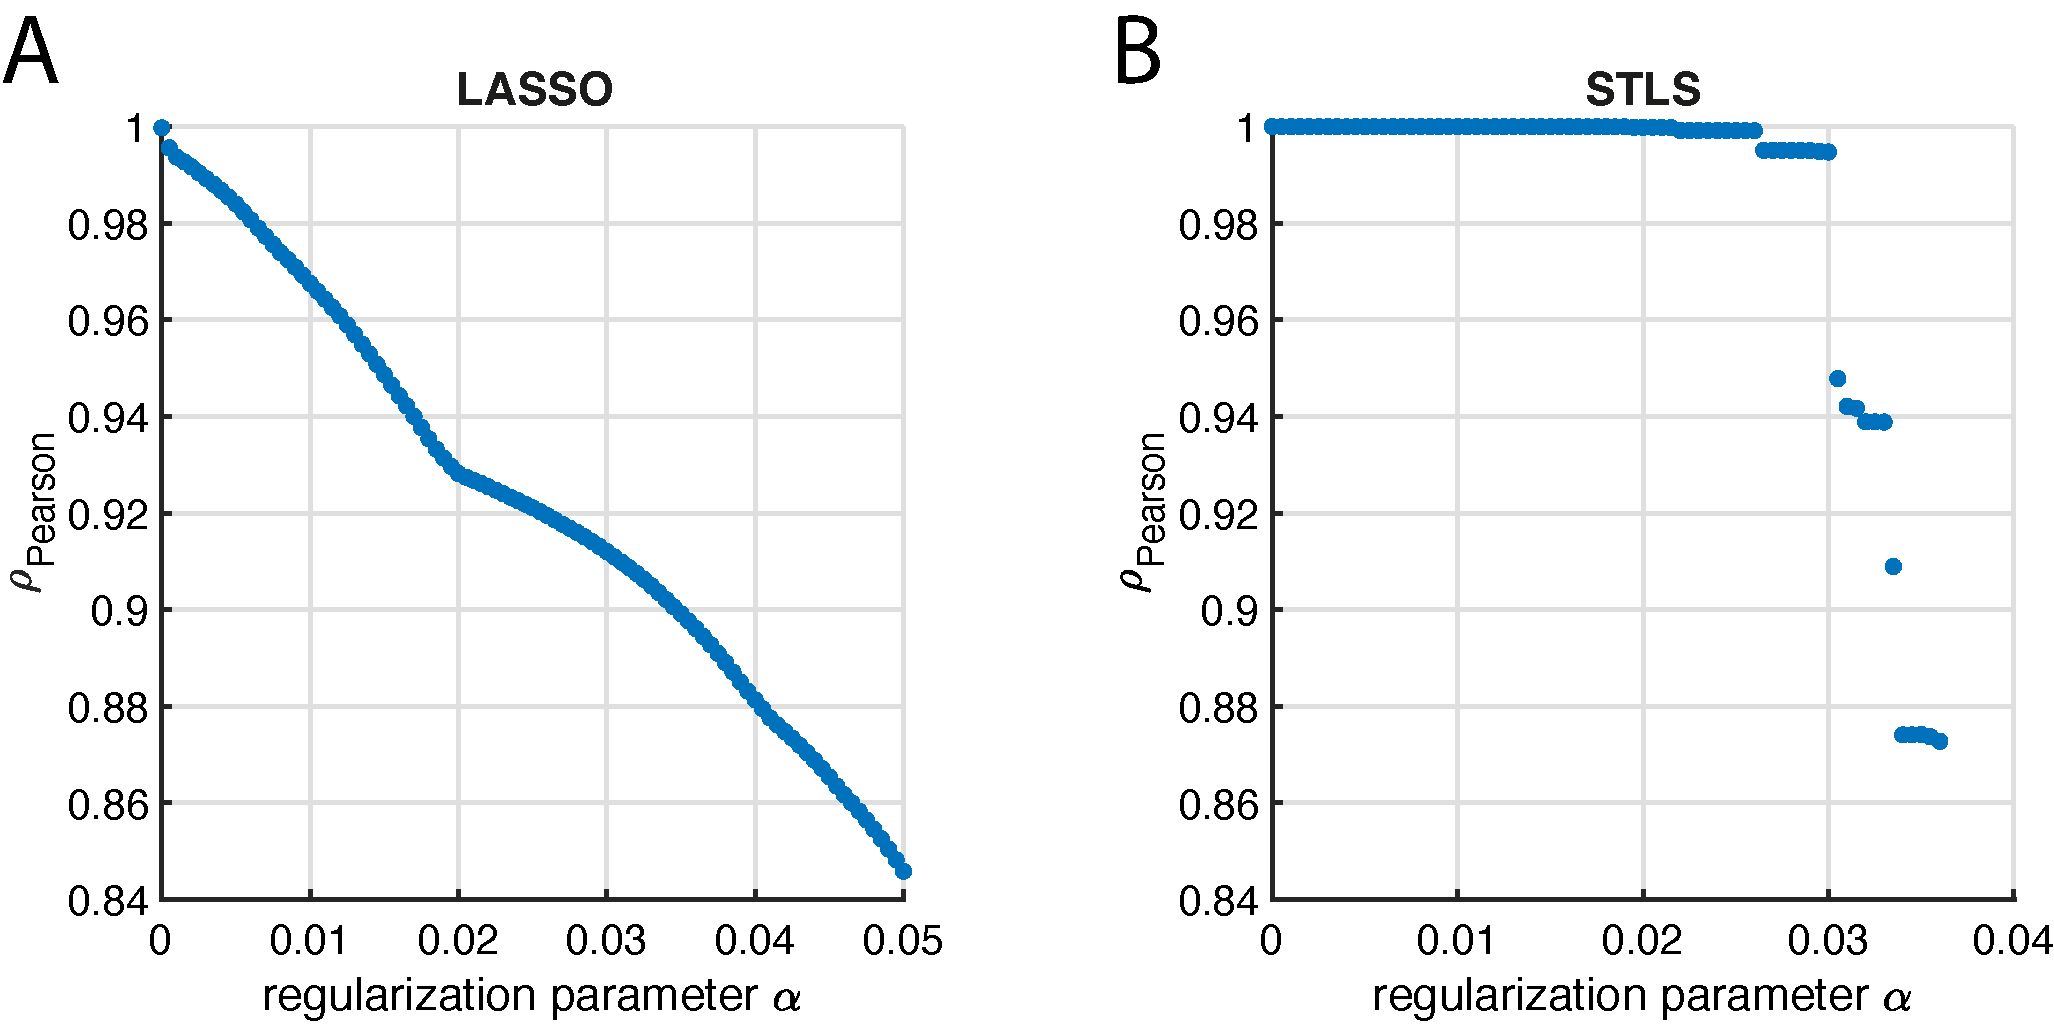
\includegraphics[width=\textwidth]{./figures/fig_regularization}
 \caption{Pearson correlation coefficient $\rho_{\vec{s},\tilde{\vec{s}}}$ between the input signal signal $\vec{s}$ and the re-composed signal $\tilde{\vec{s}}=\bfX^T\hat{\boldsymbol\beta}$ as a 
 function of the regularization parameter $\alpha$ for \textbf{A} LASSO and \textbf{B} sequentially thresholded least squares (STLS) regression (see also Section \ref{sec_tau_rr_method}). 
 The input time series is of length $N=200$ and stems from the $\tau$-RR of R\"ossler system in regular dynamics.}
\label{fig_regularization}
\end{figure}

%%%%%%%%%%%%%%%%%%%%%%%%%%%%%%%%%%%%%%%%%%
\begin{adjustwidth}{-\extralength}{0cm}
%\printendnotes[custom] % Un-comment to print a list of endnotes


\reftitle{References}

% References, variant A: external bibliography

%\bibliography{your_external_BibTeX_file}
% BibTeX users please use one of
%\bibliographystyle{spbasic}      % basic style, author-year citations
%\bibliographystyle{spmpsci}      % mathematics and physical sciences
%\bibliographystyle{spphys}       % APS-like style for physics
%\bibliography{}   % name your BibTeX data base

%\bibliographystyle{spbasic} 
\bibliography{inter_spike_bib}

% If authors have biography, please use the format below
%\section*{Short Biography of Authors}
%\bio
%{\raisebox{-0.35cm}{\includegraphics[width=3.5cm,height=5.3cm,clip,keepaspectratio]{Definitions/author1.pdf}}}
%{\textbf{Firstname Lastname} Biography of first author}
%
%\bio
%{\raisebox{-0.35cm}{\includegraphics[width=3.5cm,height=5.3cm,clip,keepaspectratio]{Definitions/author2.jpg}}}
%{\textbf{Firstname Lastname} Biography of second author}

% For the MDPI journals use author-date citation, please follow the formatting guidelines on http://www.mdpi.com/authors/references
% To cite two works by the same author: \citeauthor{ref-journal-1a} (\citeyear{ref-journal-1a}, \citeyear{ref-journal-1b}). This produces: Whittaker (1967, 1975)
% To cite two works by the same author with specific pages: \citeauthor{ref-journal-3a} (\citeyear{ref-journal-3a}, p. 328; \citeyear{ref-journal-3b}, p.475). This produces: Wong (1999, p. 328; 2000, p. 475)

%%%%%%%%%%%%%%%%%%%%%%%%%%%%%%%%%%%%%%%%%%
%% for journal Sci
%\reviewreports{\\
%Reviewer 1 comments and authors’ response\\
%Reviewer 2 comments and authors’ response\\
%Reviewer 3 comments and authors’ response
%}
%%%%%%%%%%%%%%%%%%%%%%%%%%%%%%%%%%%%%%%%%%
\end{adjustwidth}
\end{document}

